\PassOptionsToPackage{table}{xcolor}
\documentclass{beamer}

\usetheme{Madrid}

%\setbeamertemplate{bibliography item}{\insertbiblabel}

\usepackage[utf8]{inputenc}
\usepackage{caption}
\usepackage{mathtools}
\usepackage{mathrsfs}
\usepackage{tabularx}
\usepackage{color, colortbl}
\usepackage{array, booktabs, ragged2e}
\usepackage{makecell}
\usepackage{tikz}
\usepackage{textpos}
% Recommended, but optional, packages for figures and better typesetting:
\usepackage{microtype}
\usepackage{graphicx}
\usepackage{subcaption}
% \usepackage{subfig}
\usepackage{booktabs} % for professional tables

\usepackage{csquotes}
\usepackage{kotex, amsmath, amssymb, amsthm, mathtools, systeme, bm, bbm, physics}
\usepackage[ruled,vlined,linesnumbered]{algorithm2e}
\usepackage{optidef}
\usepackage{arydshln}
\usepackage[table]{xcolor}
\usepackage{multicol}
\usepackage{float}
\usepackage{inputenc}

\usepackage{hyperref}

%\newlist{enumthm}{enumerate}{1}
%\setlist[enumthm]{label=(\Alph*)}
\newcommand*{\theorembreak}{\usebeamertemplate{theorem end}\framebreak\usebeamertemplate{theorem begin}}

\definecolor{RowColorOdd}{rgb}{0.914,0.914,0.953}
\definecolor{RowColorEven}{rgb}{1,1,1}

\definecolor{lightgray}{rgb}{0.83, 0.83, 0.83}

\renewcommand\theadfont{\bfseries}

\DeclareMathOperator{\balance}{balance}
\DeclareMathOperator{\argmin}{argmin}

\SetKwInput{KwInput}{Input}
\SetKwInput{KwOutput}{Output}

\newtheorem{proposition}{Proposition}

\newtheorem{remark}{Remark}
\newtheorem{assumption}{Assumption}


% Information for title page:
\title[Fair PCA]
{Fast and Efficient Fair PCA via Optimization over Stiefel Manifold}

\subtitle{}
\author[Junghyun Lee]
{Junghyun Lee\inst{1}, Gwangsu Kim\inst{2}, Matt Olfat\inst{3,4}, Mark Hasegawa-Johnson\inst{5}, Chang D. Yoo\inst{2}}

\institute[KAIST]
{
	\inst{1}%
	Graduate School of AI, KAIST
	\and
	\inst{2}%
	School of Electrical Engineering, KAIST
	\and
	\inst{3}%
	UC Berkeley
	\and
	\inst{4}%
	Citadel
	\and
	\inst{5}%
	Department of Electrical and Computer Engineering, UIUC
}

\date[ECE 590SIP @ UIUC (Fair PCA)]{\today}


%------------------------------------------------------------
%The next block of commands puts the table of contents at the 
%beginning of each section and highlights the current section:

\AtBeginSection[]
{
	\begin{frame}
		\frametitle{Outline}
		\tableofcontents[currentsection]
	\end{frame}
}

\AtBeginSubsection[]
{
	\begin{frame}
		\frametitle{Outline}
		\tableofcontents[currentsection, currentsubsection]
	\end{frame}
}
%------------------------------------------------------------

\begin{document}
	\frame{\titlepage}
	
	\tableofcontents
	
	\section{Introduction}

	\begin{frame}
	\frametitle{Fair Machine Learning}
		\begin{itemize}
			\item An active area of research with enormous societal impact
			
			\item Machine learning algorithms should not be dependent on specific (sensitive) variables such as gender, age, race...etc.
			
			\item There are multiple frameworks on how to do this:
			\begin{itemize}
				\item {\bf Fair supervised learning}
				\item Fair unsupervised learning
				\item {\bf Fair representation learning}
				\item Fair data preprocessing
				\item ...etc.
			\end{itemize}
		\end{itemize}
	\end{frame}

	\begin{frame}
	\frametitle{Fair Supervised Learning}
		\begin{itemize}
			\item We briefly review three of the most widely-used definitions of fairness in supervised learning, as formulated in \cite{Madras18a}.
			
			\item $(Z, Y, A)\in \mathbb{R}^d \times \{0,1\} \times \{0, 1\}$: joint distribution of the dimensionality-reduced data, (downstream task) label, and protected attribute.
			
			\item $g : \mathbb{R}^d \rightarrow \{0, 1\}$: classifier that outputs prediction $\hat{Y}$ for $Y$ from $Z$.
					
			\item $D_s$: probability measure of $Z_s \triangleq Z | A = s$ for $s \in \{0, 1\}$
			
			\item $D_{s, y}$: probability measure of $Z_s \triangleq Z | A = s, Y= y$ for $s, y \in \{0, 1\}$.
		\end{itemize}
	\end{frame}

	\begin{frame}
	\frametitle{Fair Supervised Learning}
		\begin{definition}[\cite{FeldmanFMSV15}]
			$g$ is said to satisfy {\bf demographic parity (DP) up to $\Delta_{DP}$} w.r.t. $A$ with 
			$\Delta_{DP} \triangleq \left| \mathbb{E}_{x \sim D_0}[g(x)] - \mathbb{E}_{x \sim D_1}[g(x)] \right|$.
		\end{definition}
		
		\begin{definition}[\cite{HardtPNS16}]
			$g$ is said to satisfy {\bf equalized opportunity (EOP) up to $\Delta_{EOP}$} w.r.t. $A$ and $Y$ with
			$\Delta_{EOP} \triangleq \left| \mathbb{E}_{x \sim D_{0, 1}}[g(x)] - \mathbb{E}_{x \sim D_{1, 1}}[g(x)] \right|$.
		\end{definition}
	
		\begin{definition}[\cite{HardtPNS16}]
			$g$ is said to satisfy {\bf equalized odds (EOD) up to $\Delta_{EOD}$} w.r.t. $A$ and $Y$ with
			$\Delta_{EOD} \triangleq \max_{y \in \{0, 1\}} \left| \mathbb{E}_{x \sim D_{0, y}}[g(x)] - \mathbb{E}_{x \sim D_{1, y}}[g(x)] \right|$.
		\end{definition}
	
	\begin{itemize}
		\item From hereon, we refer to such $\Delta_{f}(g)$ as the {\bf fairness metric of $f \in \{DP, EOP, EOD\}$ w.r.t. $g$}, respectively.
	\end{itemize}
	\end{frame}


	\begin{frame}
	\frametitle{Fair Representation Learning}
	\begin{itemize}
		\item ``Representation learning is a promising approach for implementing algorithmic
		fairness" \cite{fair-representation-tutorial}
		
		\item In this framework, a modular separation between roles can be made:
		\begin{itemize}
			\item data regulator
			\item data producer
			\item data user
		\end{itemize}
		
		\item This has several positive implications:
		\begin{itemize}
			\item centralize fairness constraints, by moving the fairness responsibility from the data user to the data regulator
			\item simplify and centralize the task of fairness auditing
			\item can be constructed to satisfy multiple fairness measures simultaneously
			\item simplify the task of evaluating the fairness/performance tradeoff, e.g., using performance bounds
		\end{itemize}
	\end{itemize}
	\end{frame}

	
	\section{Review of FPCA}
	\begin{frame}
	\frametitle{Two Notions of Fair PCA}
		\begin{itemize}
			\item There are two branches of works on ensuring fairness in PCA, each of which considers a completely {\it different} definition of fairness:
			\begin{itemize}
				\item The reconstruction errors of two (or more) sensitive groups should be similar i.e. one group's reconstruction error should not be significantly higher than others. \cite{SamadiTMSV18, TantipongpipatS19}
				
				\item The distribution of two sensitive groups should be similar i.e. an adversary should not be able to distinguish between the two groups, after the PCA \cite{OA19, Lee21}
			\end{itemize}
		\end{itemize}
	\end{frame}

	\begin{frame}
	\frametitle{Two Notions of Fair PCA}
		\begin{itemize}
			\item It turns out that these two definitions conflict with one another:
		\end{itemize}
		\begin{figure}
			\centering
			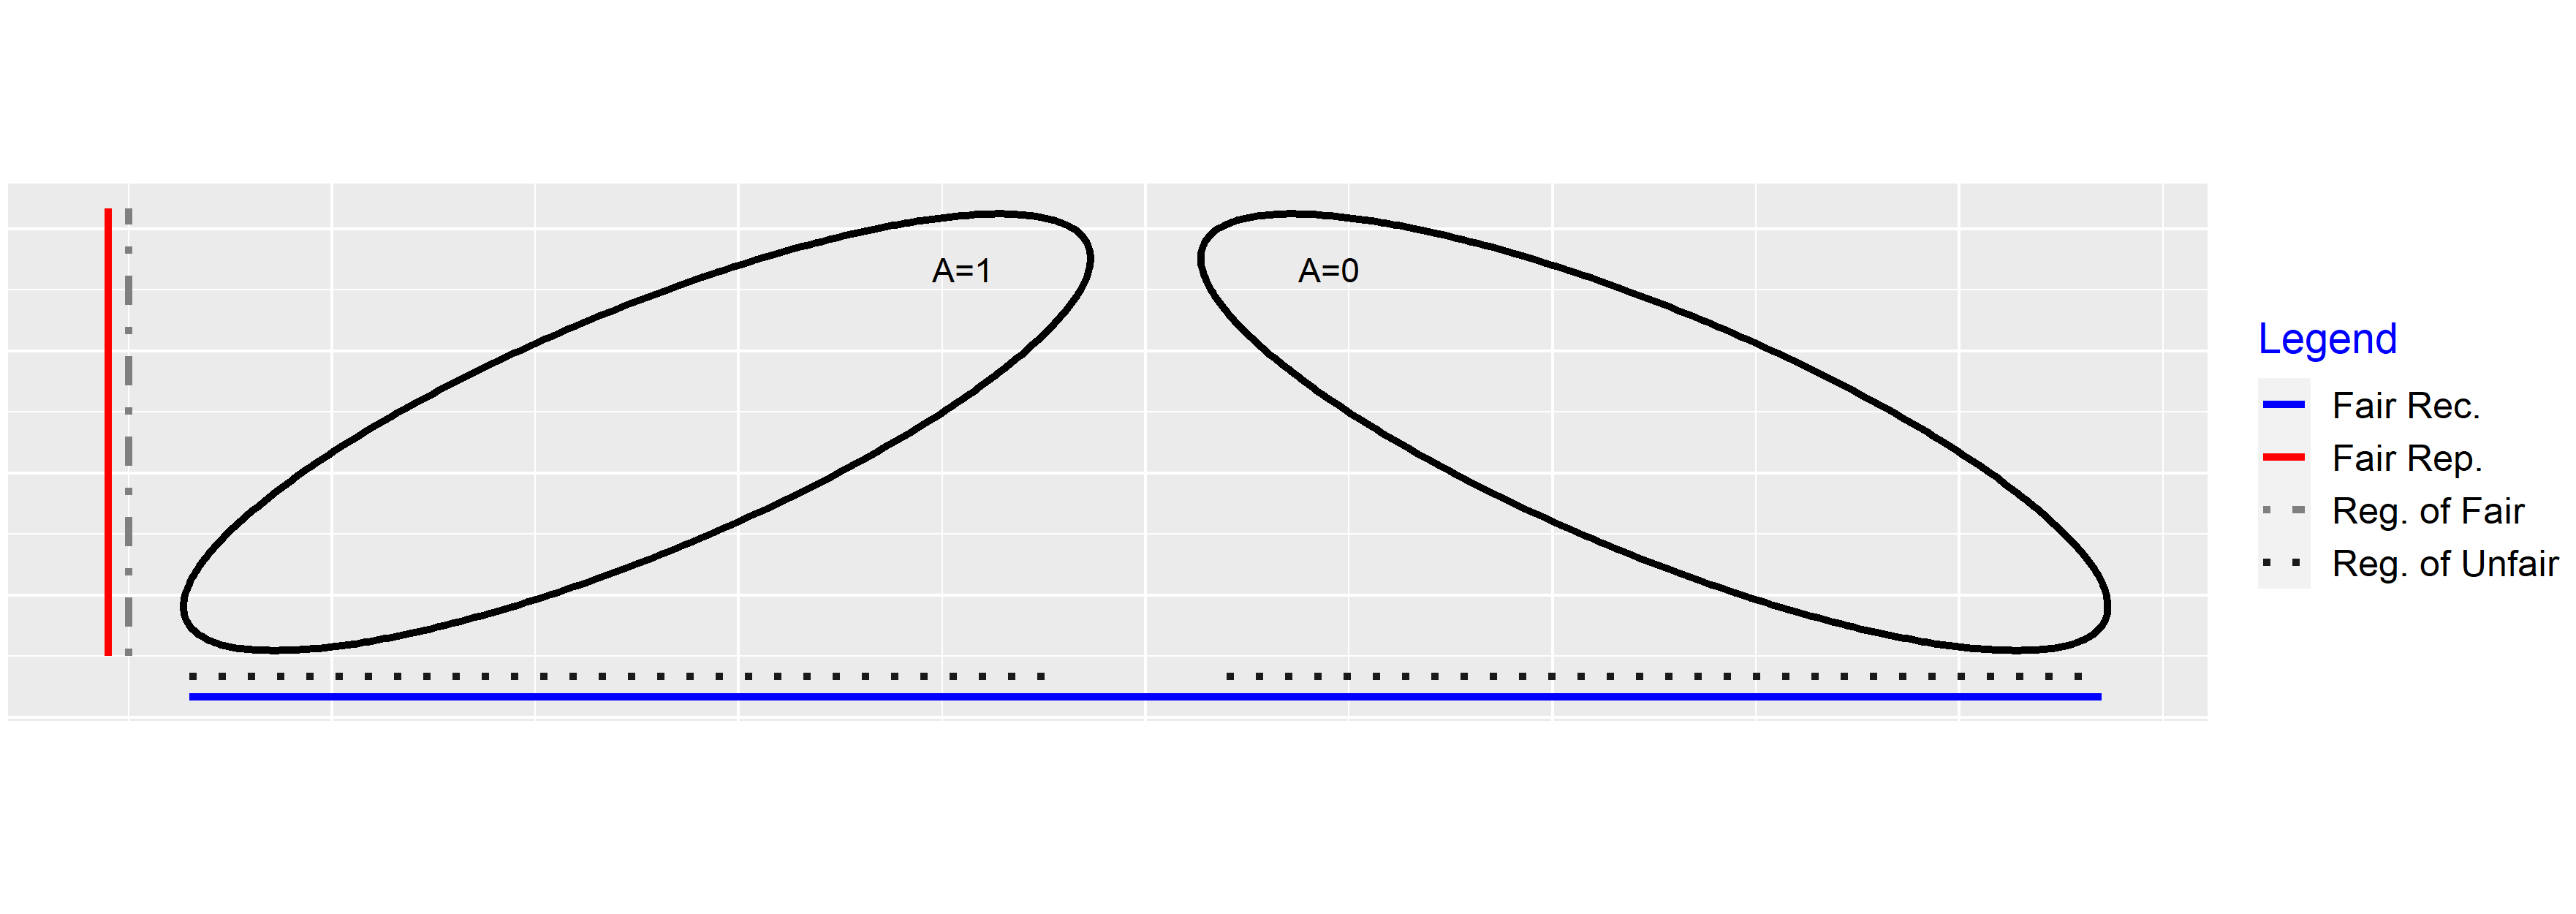
\includegraphics[width=\linewidth]{figures/comp.png}
			\caption{A toy example demonstrating how the two different definitions of fair PCA conflict with one another \cite{Lee21}}
			\label{fig:comparison1}
		\end{figure}
	\end{frame}

	\begin{frame}
	\frametitle{Adversarial Definition: FPCA}
	\begin{itemize}
		\item Here, we consider the latter notion regarding the distribution similarity after PCA.
		
		\item To motivate our work, we first review the work by Olfat \& Aswani \cite{OA19} that first considered this problem of fair PCA:
	\end{itemize}

	\begin{definition}[$\Delta_A$-fairness, \cite{OA19}]
		\label{def:delta-fairness}
		Consider a fixed classifier $h(u, t): \mathbb{R}^d \times \mathbb{R} \rightarrow \{0, 1\}$ that inputs features $u \in \mathbb{R}^d$ and a threshold $t$, and predicts the protected class $z \in \{0, 1\}$.
		Then, a dimensionality reduction $\Pi: \mathbb{R}^p \rightarrow \mathbb{R}^d$ is  $\Delta_A(h)$-fair if
		\begin{equation}
			\Big| \mathbb{P}\big[ h(\Pi(x), t) = 1 | z = 1 \big] - \mathbb{P}\big[ h(\Pi(x), t) = 1 | z = 0 \big] \Big| \leq \Delta_A(h), \ \forall t \in \mathbb{R}.
		\end{equation}
		
		Moreover, for a family of classifiers $\mathcal{F}$, if $\Pi$ is $\Delta_A(h)$-fair for $\forall h \in \mathcal{F}$, we say that $\Pi$ is $\Delta_A(\mathcal{F})$-fair.
	\end{definition}
	\end{frame}

	\begin{frame}
	\frametitle{Adversarial Definition: FPCA}
		\begin{itemize}
			\item The classifiers in the definition are {\bf adversarial}; they try to classify the protected class from the dimensionality-reduced data.
			
			\item Them performing poorly is an indicator of being fair.
		\end{itemize}
	\begin{figure}
		\centering
		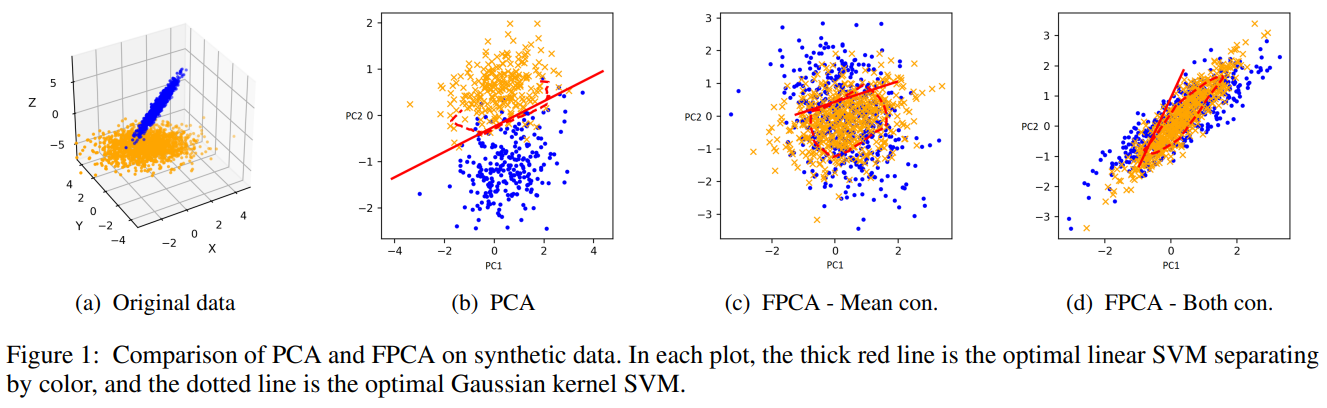
\includegraphics[width=\linewidth]{figure2}
		\caption{When vanilla PCA is applied to (a), an unfair dimensionality-reduced representation (b) is obtained. By constraining the PCA with appropriate fairness constraints, we obtain a fair representation (d). (From \cite{OA19})}
		\label{fig:figure2}
	\end{figure}
	\end{frame}

	\begin{frame}
	\frametitle{Estimator for $\Delta(\mathcal{F})$}
	\begin{itemize}
		\item With a slight abuse of notation, let
		\begin{equation*}
			\Delta_A(h) := \sup_{t \in \mathbb{R}} \Big| \mathbb{P}\big[ h(\Pi(x), t) = 1 | z = 1 \big] - \mathbb{P}\big[ h(\Pi(x), t) = 1 | z = 0 \big] \Big|
		\end{equation*}
		
		and
		\begin{equation*}
			\Delta_A(\mathcal{F}) := \sup_{h \in \mathcal{F}} \Delta(h)
		\end{equation*}
		
		\item For the actual computation, they proposed the following estimator:
		\begin{equation*}
			\widehat{\Delta}(h) = \sup_t \left| \frac{1}{|P|} \sum_{i \in P} I_i(\Pi, h_t) - \frac{1}{|N|} \sum_{i \in N} I_i(\Pi, h_t) \right|, \ \ \widehat{\Delta}(\mathcal{F}) = \sup_{h \in \mathcal{F}} \widehat{\Delta}(h)
		\end{equation*}
		where $\{x_i\}_{i=1}^n$ are the data points, $(P, N)$ is a partition of the index set $[n] := \{1, 2, \dots, n\}$ into two sensitive groups, and $I_i(\Pi, h_t) = {\bf 1}(h(\Pi(x_i), t) = 1)$.
		Here, ${\bf 1}(\cdot)$ is the indicator function.
		
	\end{itemize}
	\end{frame}

	\begin{frame}
		\frametitle{Fairness Constraints}
		\begin{itemize}
			\item For PCA, $\Pi(x) = V^\intercal x$ for some $V \in \mathbb{R}^{p \times d}$ such that $V^\intercal V = \mathbb{I}$.
			
			\item Under {\bf\color{red} Gaussian assumption}, \cite{OA19} derived the following fairness constraints:
			\begin{itemize}
				\item {\it Mean constraint}:
				\begin{equation*}
					h_{mean}(V) := \lVert V^\intercal (\mu_1 - \mu_0) \rVert = 0
				\end{equation*}
	
				\item {\it Covariance constraint}:
				\begin{equation*}
					h_{cov}(V) := \lVert V^\intercal (\Sigma_1 - \Sigma_0) V \rVert_2 = 0
				\end{equation*}
			\end{itemize}
		
			\item The derivation is, however, {\bf\color{red} complicated (not straightforward from Definition \ref{def:delta-fairness})} in the sense that several inequalities (e.g. Pinsker's inequality) had to be utilized.
		\end{itemize}
	\end{frame}

	\begin{frame}
	\frametitle{Fairness Constraints}
		\begin{itemize}
			\item For simplicity, let us denote $f := \mu_1 - \mu_0$ and $Q := \Sigma_1 - \Sigma_0$.
			
			\item Then the fair PCA can be written as a {\it constrained optimization} :
			\begin{equation}
				\label{eq:FPCA}
				\begin{aligned}
					& \underset{V}{\text{maximize}}
					& &  %f(V) := 
					\left\langle \frac{1}{n} X^\intercal X, V V^\intercal \right\rangle\\
					& \text{subject to}
					& & V^\intercal V = \mathbbm{I}_d, \\
					&&& h_{mean}(V) = 0, \\
					&&& h_{cov}(V) = 0.
				\end{aligned}
			\end{equation}
			
			\begin{itemize}
				\item $\frac{1}{n} X^\intercal X$: (total) covariance matrix of the original data matrix $X \in \mathbb{R}^{n \times p}$
				
				\item $\left\langle \frac{1}{n} X^\intercal X, V V^\intercal \right\rangle$: {\it explained variance} of $X$ after applying (linear) PCA using $V$.
			\end{itemize}			
		\end{itemize}
	\end{frame}

	\begin{frame}
	\frametitle{SDP Formulation of Fair PCA}
	\begin{itemize}
		\item \cite{OA19} provided a SDP formulation of above optimization\footnote{This was heavily inspired from the SDP formulation of vanilla PCA \cite{ACS13}.}:
		\begin{figure}
			\centering
			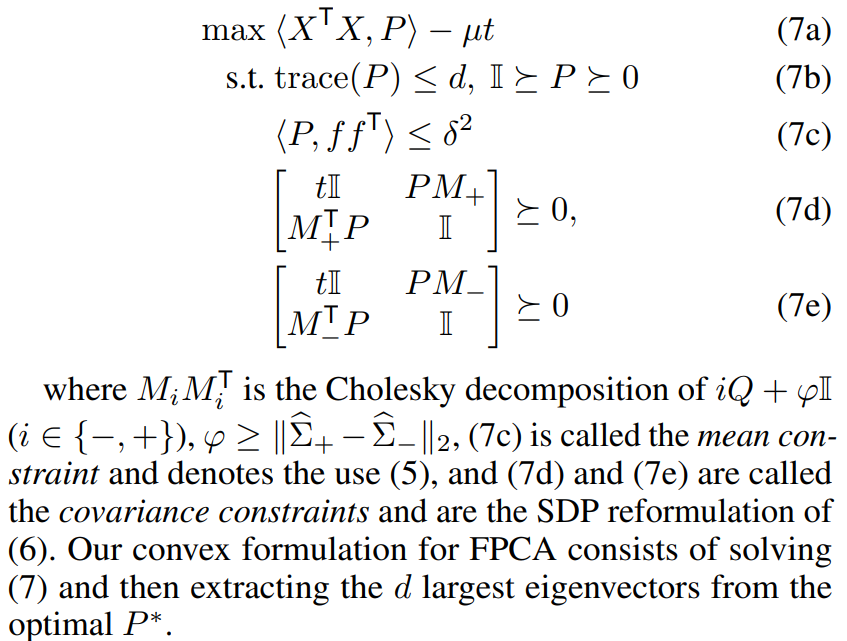
\includegraphics[width=0.6\linewidth]{sdp}
			\caption{$\delta$: bound for mean difference, $\mu$: bound for covariance difference}
			\label{fig:sdp}
		\end{figure}
	\end{itemize}
	\end{frame}

%---------------------------------------------------------

\section{Problems with FPCA}

\begin{frame}
	\frametitle{Problems with FPCA}
	\begin{itemize}
		\item There are two parts to this section.
		
		\item First subsection is devoted to show the limitation of the $\Delta_A$-fairness definition itself.
		
		\item Second subsection is devoted to show the limitation of the numerical algorithm, namely the SDP.
	\end{itemize}
\end{frame}

\subsection{Problems with the definition}

\begin{frame}
	\frametitle{Computational Inefficiency}
	\begin{itemize}
		\item Recall the definition of $\widehat{\Delta}_A$:
		\begin{equation*}
			\widehat{\Delta}_A(\mathcal{F}_c) = \sup_{h \in \mathcal{F}_c} \sup_t \left| \frac{1}{|P|} \sum_{i \in P} I_i(\Pi, h_t) - \frac{1}{|N|} \sum_{i \in N} I_i(\Pi, h_t) \right|
		\end{equation*}
		
		\item Computing above requires considering all possible classifiers in the designated family $\mathcal{F}_c$, and all possible thresholds $t \in \mathbb{R}$.
		
		\item This is computationally infeasible, and it forces one to use another approximation (e.g. discretization of $\mathcal{F}_c$), which incurs additional error that may further inhibit asymptotic consistency.
	\end{itemize}
\end{frame}

\begin{frame}
	\frametitle{Asymptotic Inconsistency}
	\begin{itemize}
		\item $\widehat{\Delta}_A$ is known to satisfy the following bound:
		\begin{proposition}[\cite{OA19}]
			Consider a fixed family of classifiers $\mathcal{F}_c$.
			Then for any $\delta > 0$, with probability at least $1 - \exp\left( - \frac{(n + m) \delta^2}{2} \right)$ the following holds:
			\begin{equation}
				\left| \Delta_A(\mathcal{F}_c) - \widehat{\Delta}_A(\mathcal{F}_c) \right| \leq 8 \sqrt{\frac{{\color{red} VC(\mathcal{F}_c)}}{m + n}} + \delta
			\end{equation}
			
			where $VC(\cdot)$ is the VC dimension.
		\end{proposition}
		
		\item If $\mathcal{F}_c$ is too expressive, then the above bound may become void!
				
		\item This is the case, for instance, when $\mathcal{F}_c$ is the set of RBF-kernel SVMs, whose VC dimension is infinite...
	\end{itemize}
\end{frame}


\subsection{Problems with the SDP}

\begin{frame}
	\frametitle{SDP Relaxation of Fair PCA}
	\begin{itemize}
		\item The orthogonality constraint $V^\intercal V = \mathbbm{I}_d$ has to be relaxed to trace bound and matrix inequalities.
		
		\item Without the fairness constraints, it can be proven that the SDP formulation exactly outputs the optimal solution to the optimization problem.
		
		\item But with the additional constraints, theoretical guarantee (for optimality) is {\bf not} available!
	\end{itemize}
\end{frame}

\begin{frame}
	\frametitle{Inscalability to High Dimensions}
	\begin{itemize}
		\item Recall that the SDP is solved w.r.t. a new variable, $P \in \mathbb{R}^{p \times p}$.
		
		\item Size of the variable scales {\it quadratically} to the original data's dimension $p$, {\it independent of the dimension $d$ to which we are reducing to}.
		
		\item Empirically we've shown that the time complexity of FPCA grows very large in $p$, even for datas with simple block-structured covariance matrices!
		
		\item In comparison, our to-be introduced manifold optimization based approach scales very well in high dimensions.
	\end{itemize}
\end{frame}

\begin{frame}
	\frametitle{Inscalability to High Dimensions}
	\begin{figure}
		\centering
		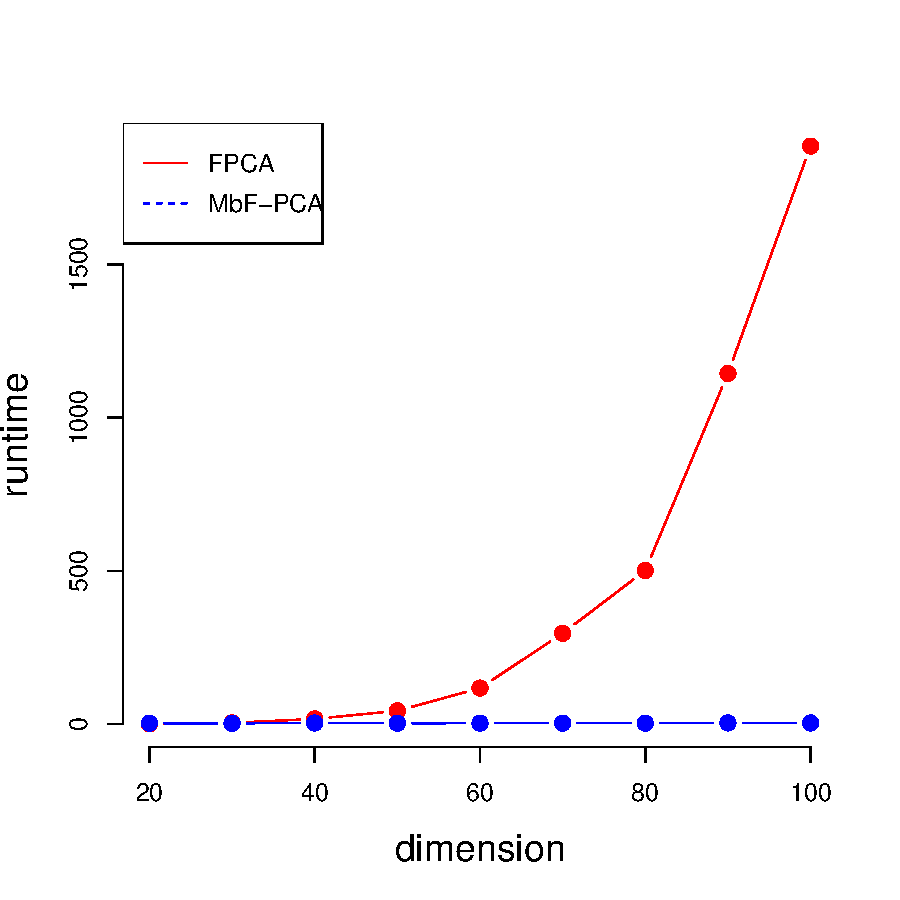
\includegraphics[width=0.5\linewidth]{figures/exp1-2/runtime.pdf}
		\caption{FPCA represents the SDP algorithm for fair PCA, and MbF-PCA represents our to-be introduced manifold-based algorithm for fair PCA. \cite{Lee21}}
		\label{fig:runtime}
	\end{figure}
\end{frame}

\begin{frame}
	\frametitle{``Counterexample'' to FPCA}
	\begin{itemize}
	\item Recall how the {\bf Gaussian assumption} was required for deriving the actual numerical algorithm.
	
	
	\item FPCA, thus, cannot cover the case when two sensitive distributions, that are different, have the same first two moments (mean, covariance):
	\end{itemize}
	
	\begin{figure}[!t]
		\begin{center}
			\begin{subfigure}[t]{0.24\linewidth}
				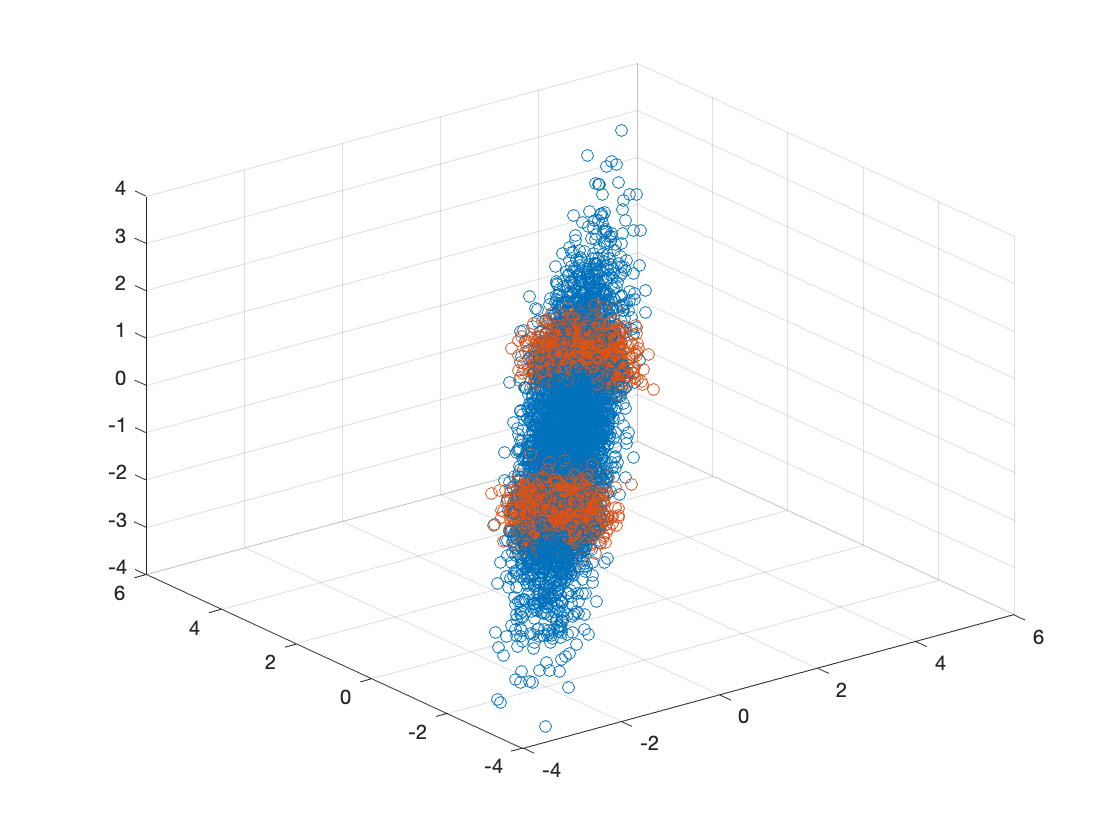
\includegraphics[width=\linewidth]{figures/exp1-1/original.png}
				\caption{\label{fig:original} Original data}
			\end{subfigure}\hfill
			\begin{subfigure}[t]{0.24\linewidth}
				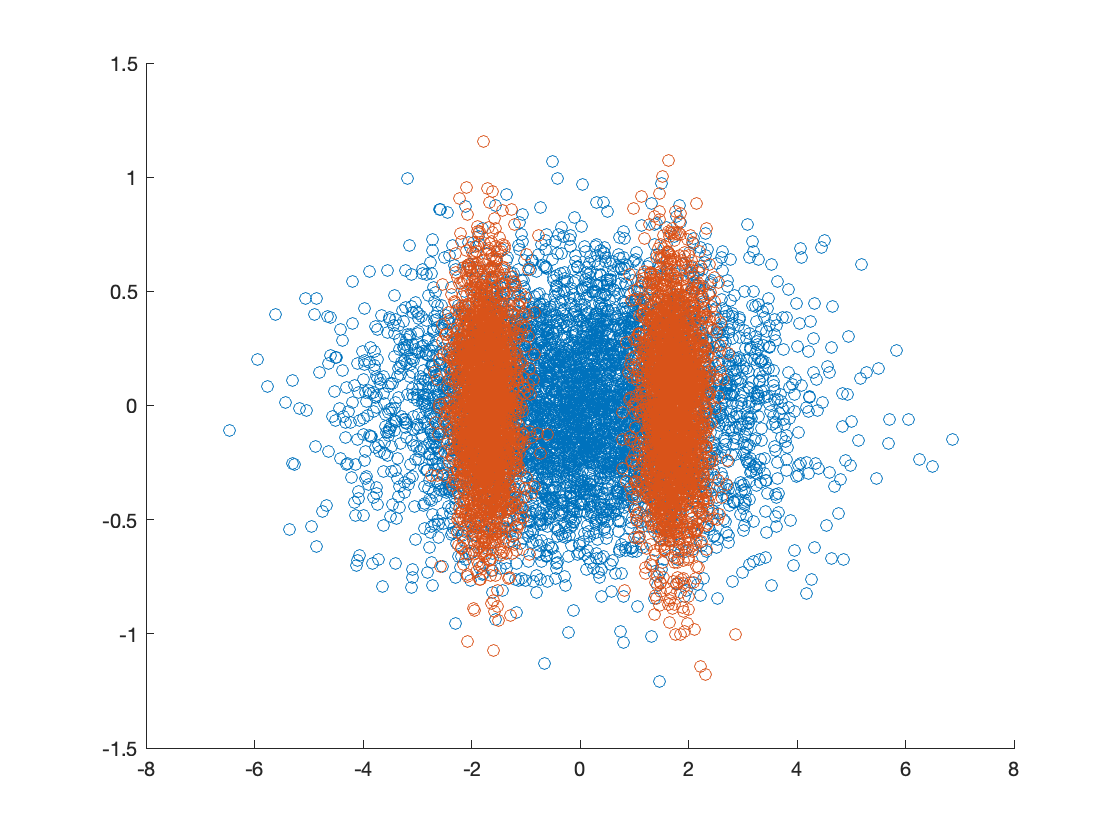
\includegraphics[width=\linewidth]{figures/exp1-1/pca.png}
				\caption{\label{fig:PCA} PCA}
			\end{subfigure}\hfill
			\begin{subfigure}[t]{0.24\linewidth}
				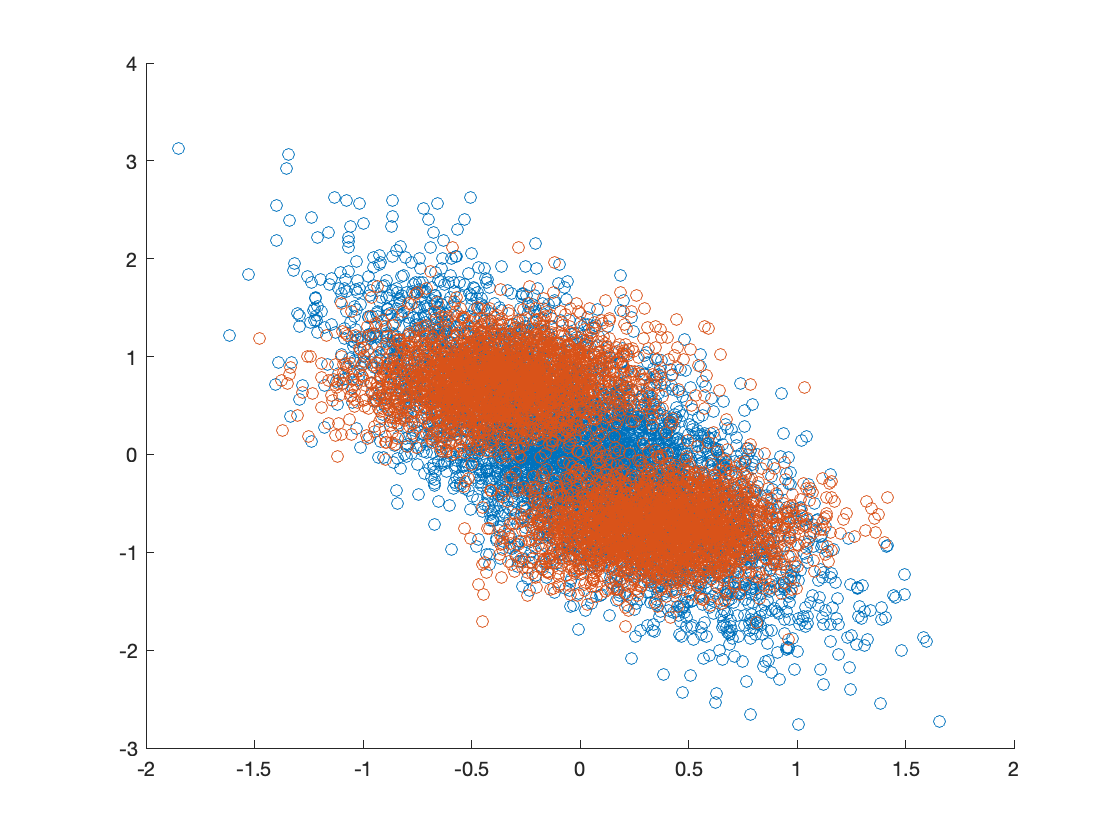
\includegraphics[width=\linewidth]{figures/exp1-1/fpca.png}
				\caption{\label{fig:FPCA} \textsc{FPCA} \cite{OA19}}
			\end{subfigure}\hfill
			\begin{subfigure}[t]{0.24\linewidth}
				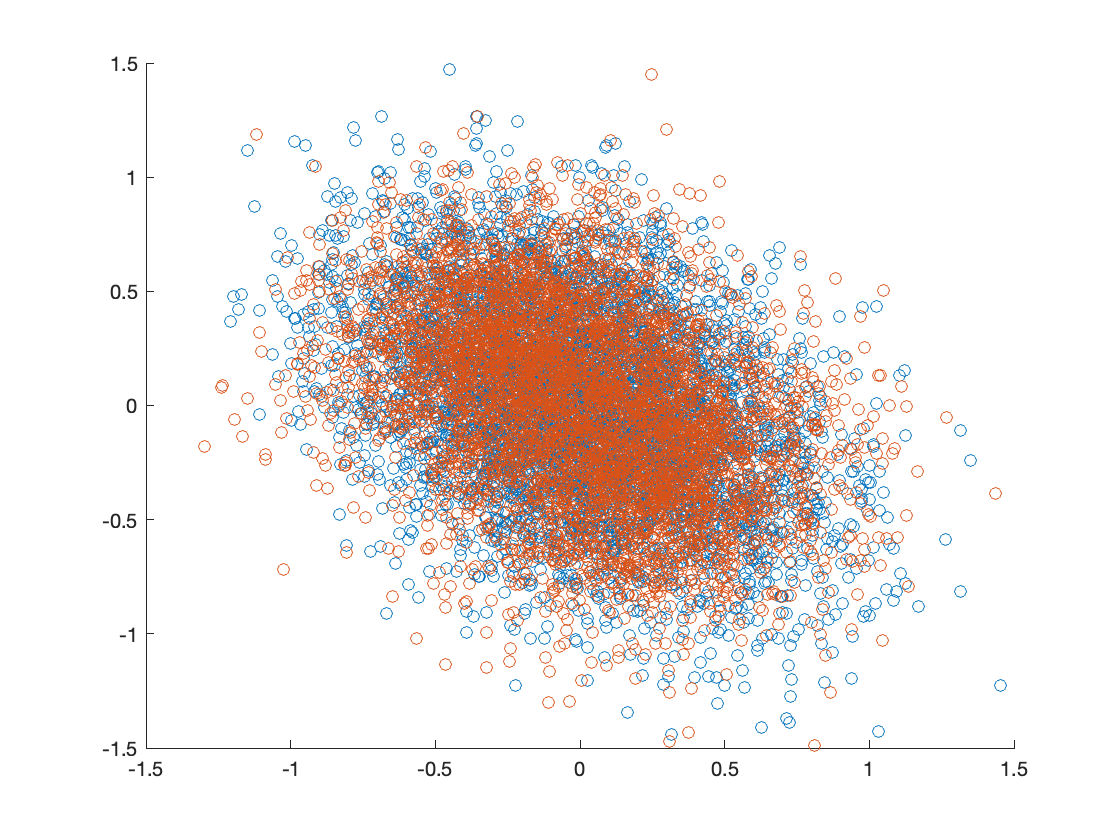
\includegraphics[width=\linewidth]{figures/exp1-1/mbfpca.png}
				\caption{\label{fig:ours} \textsc{MbF-PCA} (ours)}
			\end{subfigure}
			\caption{\label{fig:exp1-1} Synthetic data \#1: Comparison of PCA, FPCA, and \textsc{MbF-PCA} on data composed of two groups with same mean and covariance, but different distributions. Blue and orange represent different protected groups.}
		\end{center}
	\end{figure}
\end{frame}



%---------------------------------------------------------
\section{New Definition: $\Delta$-fairness}

\begin{frame}
	\frametitle{Quick Review of MMD}
	\begin{itemize}
		\item One way to define distance between two probability measures is as follows:	\begin{definition}[\cite{Gretton07a}]
			Given $\mu, \nu \in \mathcal{P}_d$, their {\bf maximum mean discrepancy (MMD)}, denoted as $MMD_k(\mu, \nu)$, is a pseudo-metric on $\mathcal{P}_d$, defined as follows:
			\begin{equation*}
				MMD_k(\mu, \nu) := \sup_{f \in \mathcal{H}_k} \left| \int_{\mathbb{R}^d} f \ d(\mu - \nu) \right|
			\end{equation*}
		\end{definition}
		
		\item $\mathcal{H}_k$ is the unit ball in the RKHS generated by some given kernel $k$.
		
		\item $\mathcal{P}_d$ is the set of all possible probability measures defined on $\mathbb{R}^d$.
	\end{itemize}
\end{frame}

\begin{frame}
	\frametitle{Quick Review of MMD}
	\begin{itemize}
		\item As our fairness constraint involves exactly matching the
		considered distributions using $MMD$, we require the property
		of $MMD_k(\mu, \nu) = 0$ implying $\mu = \nu$:
		\begin{definition}[\cite{Fukumizu08}]
			If $MMD_k$ metrizes $\mathcal{P}_d$, then the kernel $k$ is said to be {\bf characteristic} to $\mathcal{P}_d$.
		\end{definition}
		
		\item Sriperumbudur et al \cite{Sriperumbudur08} defined and characterized {\it stationary} characteristic kernels and identified that well-known kernels such as RBF and Laplace are characteristic.
		
		\item From hereon, we set $k$ to be the RBF kernel $k_{rbf}(x, y) := \exp(-\lVert x - y \rVert^2 / 2\sigma^2)$.
	\end{itemize}
\end{frame}

\begin{frame}
	\frametitle{Benefits of MMD}
	\begin{itemize}
		\item It can act as a distance between distributions with different, or even disjoint, supports. (unlike, for instance, KL-divergence)
		\begin{itemize}
			\item This is especially crucial as the empirical distributions are often discrete and completely disjoint.
		\end{itemize}
		
		\item Since many problems in fairness involve comparing two distributions, $MMD$ has already been used in much of the fairness literature as a metric \cite{Madras18a, Adel19} and as an explicit constraint/penalty \cite{Quadrianto17, Louizos16, Prost19, Oneto20, Jung21}, among other usages.
	\end{itemize}
\end{frame}

\begin{frame}
	\frametitle{$\Delta$-fairness}
	\begin{itemize}
		\item Motivated from previous discussions, we propose a new definition for fair PCA based on MMD:
		\begin{definition}[$\Delta$-fairness, \cite{Lee21}]
			\label{def:fairness}
			Let $P_s$ be the probability measure of $X_s \triangleq X | A = s$ for $s \in \{0, 1\}$, and let $Q_s := \Pi_\# P_s \in \mathcal{P}_d$.
			Then $\Pi$ is said to be {\bf $\Delta$-fair} with $\Delta := MMD(Q_0, Q_1)$, and we refer to $\Delta$ as the {\bf fairness metric}.
		\end{definition}
		
		\item Indeed, as every fair representation should satisfy, our definition also ensures that any {\it unconstrained} downstream tasks will also be fair:
		\begin{proposition}[\cite{Oneto20}, informal]
			\label{prop:fair-representation}
			Up to a constant factor, $MMD(Q_0, Q_1)$ bounds the MMD of the push-forward measures of $Q_0, Q_1$ via the weight vector of any given downstream task classifier $g$.
		\end{proposition}
	\end{itemize}
\end{frame}

\begin{frame}
	\frametitle{Computational Efficiency}
	\begin{itemize}
		\item We consider the following estimator:
		\begin{equation}
			\widehat{\Delta} := MMD(\hat{Q}_0, \hat{Q}_1)
		\end{equation}
		where $\hat{Q}_s$ is the usual empirical distribution, defined as the mixture of Dirac measures on the samples.
		
		\item Unlike $\widehat{\Delta}_A$, $\widehat{\Delta}$ can be computed exactly and efficiently:
		\begin{lemma}[\cite{Gretton07a}]
			\label{def:lem-computable}
			$\widehat{\Delta}$ is computed as follows:
			\begin{equation}
					\widehat{\Delta} = \Bigg[ \frac{1}{m^2} \sum_{i,j = 1}^m k(X_i, X_j) + \frac{1}{n^2} \sum_{i,j = 1}^n k(Y_i, Y_j) 
					- \frac{2}{mn} \sum_{i, j = 1}^{m, n} k(X_i, Y_j) \Bigg]^{1/2}.
			\end{equation}
		\end{lemma}
	\end{itemize}
\end{frame}

\begin{frame}
	\frametitle{Asymptotic Consistency}
	\begin{itemize}
		\item Unlike $\widehat{\Delta}_A$, $\widehat{\Delta}$ is asymptotic convergent, with the rate depending only on $m$ and $n$:
		\begin{theorem}[\cite{Gretton07a}]
			For any $\delta > 0$, with probability at least $1 - 2\exp\left(-\frac{\delta^2 mn}{2(m + n)}\right)$ the following holds:
			\begin{equation}
				\left| \Delta - \widehat{\Delta} \right| \leq 2 \left( \frac{1}{\sqrt{m}} + \frac{1}{\sqrt{n}} \right) + \delta
			\end{equation}
		\end{theorem}
	\end{itemize}
\end{frame}

\begin{frame}
	\frametitle{Relation to $\Delta_A$-fairness (*)}
	\begin{itemize}
		\item It can be argued that, for some choice of $\mathcal{F}_c$, the adversarial definition \cite{OA19} and our definition are equivalent: in effect, that these are dual notions.
		
		\item Recognizing this, we proceed with ours, as it has two main advantages in the context of our work:
		\begin{itemize}
			\item It ties more directly and intuitively into our optimization formulation, as we'll see later.
			
			\item It can be represented non-variationally %(having no supreme) ,
			which allows for tighter statistical guarantees.
		\end{itemize}
	\end{itemize}
\end{frame}

%---------------------------------------------------------
\section{New Framework: MbF-PCA}

\begin{frame}
	\frametitle{Fair PCA as Manifold Optimization}
	\begin{itemize}
		\item All the problems mentioned previously can be resolved by optimizing {\bf directly} for $V$!
		
		\item But then, this becomes a non-convex optimization problem over $\mathbb{R}^{p \times d}$ with $2$ constraints!
		\begin{itemize}
			\item Orthogonality constraint:
			\begin{equation*}
				V^\intercal V = \mathbbm{I}_d
			\end{equation*}
		
			\item Fairness constraint:
			\begin{equation*}
				h(V) := MMD^2(\hat{Q}_0, \hat{Q}_1) = 0
			\end{equation*}
		\end{itemize}
	\end{itemize}
\end{frame}

\begin{frame}
	\frametitle{Fair PCA as Manifold Optimization}
	\begin{itemize}
		\item The set of all $V$'s with $V^\intercal V = \mathbbm{I}_d$ has the intrinsic geometric structure of a {\it (matrix) manifold}:
		\begin{definition}
			For $p \geq d$, the Stiefel manifold, denoted as $St(p, d)$, is an embedded Riemannian sub-manifold of $\mathbb{R}^{p \times d}$ such that each element of $St(p, d)$ has orthonormal columns i.e. $V^\intercal V = \mathbbm{I}_d$ for all $V \in St(p, d)$. 
		\end{definition}
		
		
		\item Main idea: instead of regarding $V^\intercal V = \mathbb{I}$ as a constraint, let's optimize {\bf on} $St(p, d)$!!
		
		\item This is the basic idea behind the framework of manifold optimization.
	\end{itemize}
\end{frame}

\begin{frame}
	\frametitle{Quick Intuition behind Manifold Optimization}
	\begin{itemize}
		\item Consider $\mathcal{M}$, an embedded Riemannian sub-manifold of $\mathbb{R}^{p \times d}$.
		
		\item Suppose we want to minimize some function $f : \mathbb{R}^{p \times d} \rightarrow \mathbb{R}$ {\it over} $\mathcal{M}$.
				
		\item If $\mathcal{M}$ is simply viewed as a subset of $\mathbb{R}^{p \times d}$, then this is a constrained optimization problem:
		\begin{equation}
			\begin{aligned}
				& \underset{V}{\text{minimize}}
				& &  f(V) \\
				& \text{subject to}
				& & V \in \mathcal{M}.
			\end{aligned}
		\end{equation}
		
		\item In this case, the optimization algorithm will make use of the canonical gradients and Hessians of $\mathbb{R}^{p \times d}$.
	\end{itemize}
\end{frame}

\begin{frame}
	\frametitle{Quick Intuition behind Manifold Optimization}
	\begin{itemize}
		\item If $\mathcal{M}$ is ``all there is", then this problem is an unconstrained optimization problem over $\mathcal{M}$.
		\begin{itemize}
			\item Consider an ant living on $\mathcal{M}$. From the universe ($\mathbb{R}^{p \times d}$), the ant is constrained on $\mathcal{M}$. But from the ant's perspective, $\mathcal{M}$ is all they have i.e. he/she would feel {\it unconstrained}!
		\end{itemize}
		
		\item In this case, the optimization algorithm will make use of the {\it Riemannian} gradients and Hessians of $\mathcal{M}$.
		
		\item By making use of the intrinsic geometry of $\mathcal{M}$, the optimization becomes much more efficient!
	\end{itemize}
\end{frame}

\begin{frame}
	\frametitle{Quick Intuition behind Manifold Optimization}
	\begin{itemize}
		\item A very straightforward way to think of this is by considering the simplest Riemannian manifold\footnote{inner product is the Frobenius product: $\langle X, Y \rangle:= \tr(X^\intercal Y)$}, $\mathbb{R}^{p \times d}$.
		
		\item When we write the optimization as
		\begin{equation}
			\begin{aligned}
				& \underset{V}{\text{minimize}}
				& &  f(V) \\
				& \text{subject to}
				& & V \in \mathbb{R}^{p \times d},
			\end{aligned}
		\end{equation}
		
		technically this is a ``constrained" optimization because we're ``constraining" $V$ to be in $\mathbb{R}^{p \times d}$.
		
		\item However, gradients and Hessian (and other geometric concepts) are derived directly from the intrinsic geometry of $\mathbb{R}^{p \times d}$ i.e. {\bf $V \in \mathbb{R}^{p \times d}$ isn't considered as a constraint.}
	\end{itemize}
\end{frame}

\begin{frame}
	\frametitle{MbF-PCA}
	\begin{itemize}
		\item Thus fair PCA can be formulated as a constrained manifold optimization problem, which we refer to as MbF-PCA:
		\begin{equation}
			\label{eq:MbF-PCA}
			\begin{aligned}
				& \underset{V \in St(p, d)}{\text{maximize}}
				& &  %f(V) := 
				\left\langle \frac{1}{n} X^\intercal X, V V^\intercal \right\rangle\\
				& \text{subject to}
				& & h(V) := MMD^2(\hat{Q}_0, \hat{Q}_1) = 0.
			\end{aligned}
		\end{equation}
		
		\item With this formulation, we now have only one constraint.
		
		\item Moreover, leveraging kernel trick, an explicit form of $\grad_V h(V)$ can be found; see Section G of the SP \cite{Lee21}.
	\end{itemize}
\end{frame}

\begin{frame}
	\frametitle{REPMS for MbF-PCA}
	\begin{itemize}
		\item To solve the optimization, we use REPMS \cite{repms}.
	\end{itemize}
	
	\begin{figure}[!t]
	\begin{center}
		\begin{subfigure}[t]{0.49\linewidth}
			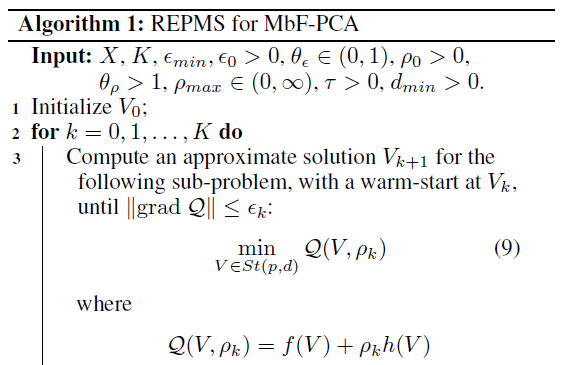
\includegraphics[width=\linewidth]{mbfpca-1}
		\end{subfigure}\hfill
		\begin{subfigure}[t]{0.49\linewidth}
			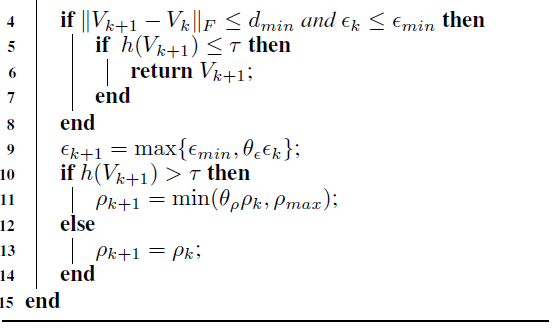
\includegraphics[width=\linewidth]{mbfpca-2}
		\end{subfigure}
		\caption{\label{alg:mbfpca} Pseudocode}
	\end{center}
\end{figure}
\end{frame}


\begin{frame}
	\frametitle{Practical Consideration}
	\begin{itemize}
		\item For practical concerns, we’ve set the fairness tolerance level, $\tau$, to be a fixed and sufficiently small, non-negative value.
		
		\item Accordingly, we consider the following definition:
		\begin{definition}
			\label{def:approx-fair}
			For fixed $\tau \geq 0$, $V \in St(p, d)$ is {\bf $\tau$-approximate fair} if it satisfies $h(V) \leq \tau$.
			If $\tau = 0$, we simply say that $V$ is {\bf fair}.
		\end{definition}
	\end{itemize}
\end{frame}


\begin{frame}
	\frametitle{New Theoretical Guarantees}
	\begin{itemize}
		\item Our problem is non-convex in $V$, which naturally brings up the question of convergence and optimality guarantees.
		
		\item First, we theoretically motivate the following assumption, which is to the best of our knowledge, new:
		\begin{assumption}[informal; locality assumption]
			\label{assumption:1}
			Each $V_{k+1}$ is sufficiently close to a local minimum of Eq. (9).
		\end{assumption}
	
		\item Also, we consider the following auxiliary optimization problem:
		\begin{equation}
			\label{eq:auxiliary}
			\min_{V \in St(p, d)} h(V)
		\end{equation}
	\end{itemize}
\end{frame}


\begin{frame}
	\frametitle{New Theoretical Guarantees}
	\begin{itemize}
		\item Our problem is non-convex in $V$, which naturally brings up the question of convergence and optimality guarantees.
		
		\item First, under {\it ideal} hyperparameter setting, we provide an exact theoretical optimality guarantee:
		\begin{theorem}
			\label{thm:mbfpca}
			Let {\color{red}\bf $K = \infty$, $\rho_{max} = \infty$, $\epsilon_{min} = \tau = 0$}, $\{V_k\}$ be the sequence generated by Alg. \ref{alg:mbfpca} under Assumption \ref{assumption:1}, and  $\overline{V}$ be any limit point of $\{V_k\}$, whose existence is guaranteed. Then the following holds:
			\begin{itemize}
				\item $\overline{V}$ is a local minimizer of Eq. \eqref{eq:auxiliary}, which is a {\color{blue} necessary condition for $\overline{V}$ to be fair}.
				
				\item {\color{blue} If $\overline{V}$ is fair}, then {$\overline{V}$ is a local minimizer of Eq. \eqref{eq:MbF-PCA}}
			\end{itemize}
		\end{theorem}
	\end{itemize}
\end{frame}

\begin{frame}
	\frametitle{New Theoretical Guarantees}
	\begin{itemize}
		\item The desired optimality guarantee is in the second bullet point, but it requires the assumption of $\overline{V}$ being fair.
		
		\item Such assumption is at least partially justified in the first bullet point in the following sense:
		\begin{itemize}
			\item The ideal hyperparameter setting of $\rho_{max} = \infty, \tau = 0, \epsilon_{min} = 0$ implies the {\it exact} local minimality of $\overline{V}$ for Eq. \eqref{eq:auxiliary}, which is in turn a {\it necessary condition} for $\overline{V}$ to be fair.
		\end{itemize}
	\end{itemize}
\end{frame}


\begin{frame}
	\frametitle{New Theoretical Guarantees}
	\begin{theorem}
		\label{thm:mbfpca-another}
		Let {\bf\color{red} $K = \infty$, $\rho_{max} < \infty$, $\epsilon_{min}, \tau > 0$}. 
		Then for any sufficiently small $\epsilon_{min}$ and  $\tilde{r} = \tilde{r}(\epsilon_{min}) > 0$,
		% 	{\color{red}
		% 	Then for some fixed $\tilde{r} > 0$ such that $\tilde{r} = r - g(\epsilon_{min})$ where $g(\epsilon_{min}) < r$},
		the following hold:
		
		\begin{itemize}
			\item $\overline{V}$ is an approximate local minimizer of Eq. \eqref{eq:auxiliary} in the sense that
			\begin{equation}
				h(\overline{V}) \leq h(V) + \beta \lVert V - \overline{V} \rVert + (\beta + L_h) g(\epsilon_{min})
			\end{equation}
			
			for all $V \in B_{\tilde{r}}(\overline{V}) \cap St(p, d)$, where $\beta = \beta(\rho_{max}, \tau)$ is a function that satisfies the following:
			\begin{itemize}
				\item $0 < \beta \leq \frac{2 \lVert \Sigma \rVert}{\rho_0}$
				
				\item $\beta(\rho_{max}, \tau)$ is increasing in $\rho_{max}$ and decreasing in $\tau$.
			\end{itemize}
		\end{itemize}
	\end{theorem}
\end{frame}

\begin{frame}
	\frametitle{New Theoretical Guarantees}
	\begin{theorem}
		\begin{itemize}
			\item If $\overline{V}$ is fair, then it is an approximate local minimizer of Eq. \eqref{eq:MbF-PCA} in the sense that it satisfies
			\begin{equation}
				f(\overline{V}) \leq f(V) + 2 \lVert \Sigma \rVert g(\epsilon_{min})
			\end{equation}
			
			for all fair $V \in B_{\tilde{r}}(\overline{V}) \cap St(p, d)$.
		\end{itemize}
		
		In both parts, $g$ is some continuous, decreasing function that satisfies $g(0) = 0$, and $\tilde{r}(\epsilon_{min}) = r - g(\epsilon_{min})$ for some fixed constant $r > 0$.
	\end{theorem}
\end{frame}


\begin{frame}
	\frametitle{Novelty of the guarantees (*)}
	\begin{itemize}
		\item Existing optimality guarantee of REPMS (Proposition 4.2; \cite{repms}) states that when $\epsilon_{min} = 0$, $\rho$ is {\it not} updated (i.e. line 10-14 is ignored), and the resulting limit point is feasible, then that limit point satisfies the KKT condition \cite{optimality-manifold}.
		
		\item Our theoretical analyses are much closer to the actual implementation, by incorporating the $\rho$-update step (line 11) and the {\it practical} hyperparameter setting.
		
		\item Our theoretical analyses are much more stronger in the sense that
		\begin{itemize}
			\item by {\it introducing} a reasonable, yet novel locality assumption, we go beyond the existing KKT conditions and prove the {\it local minimality} of the limit point.
			
			\item we provide a partial justification of the feasibility assumption in the first bullet point by proving a necessary condition.
		\end{itemize}
	\end{itemize}
\end{frame}

%---------------------------------------------------------
\section{Experiments}

\begin{frame}
	\frametitle{Synthetic data \#1}
	\begin{figure}[!t]
		\begin{center}
			\begin{subfigure}[t]{0.24\linewidth}
				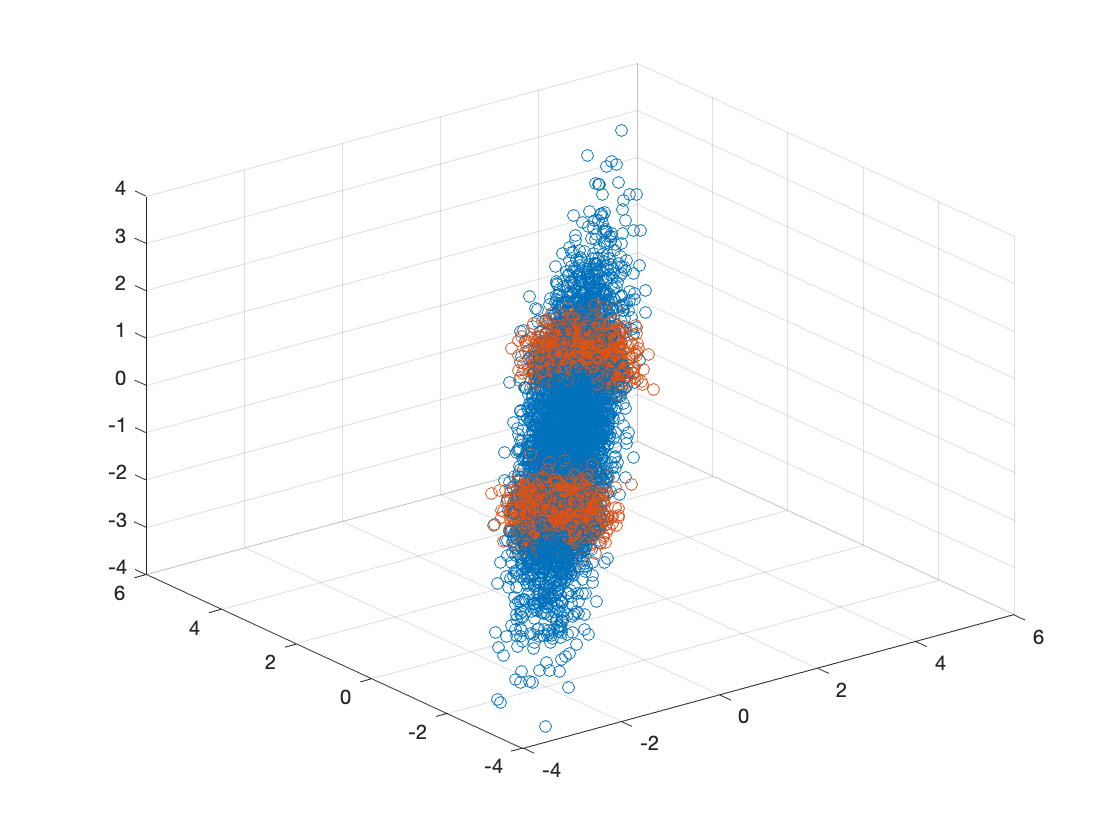
\includegraphics[width=\linewidth]{figures/exp1-1/original.png}
				\caption{\label{fig:original} Original data}
			\end{subfigure}\hfill
			\begin{subfigure}[t]{0.24\linewidth}
				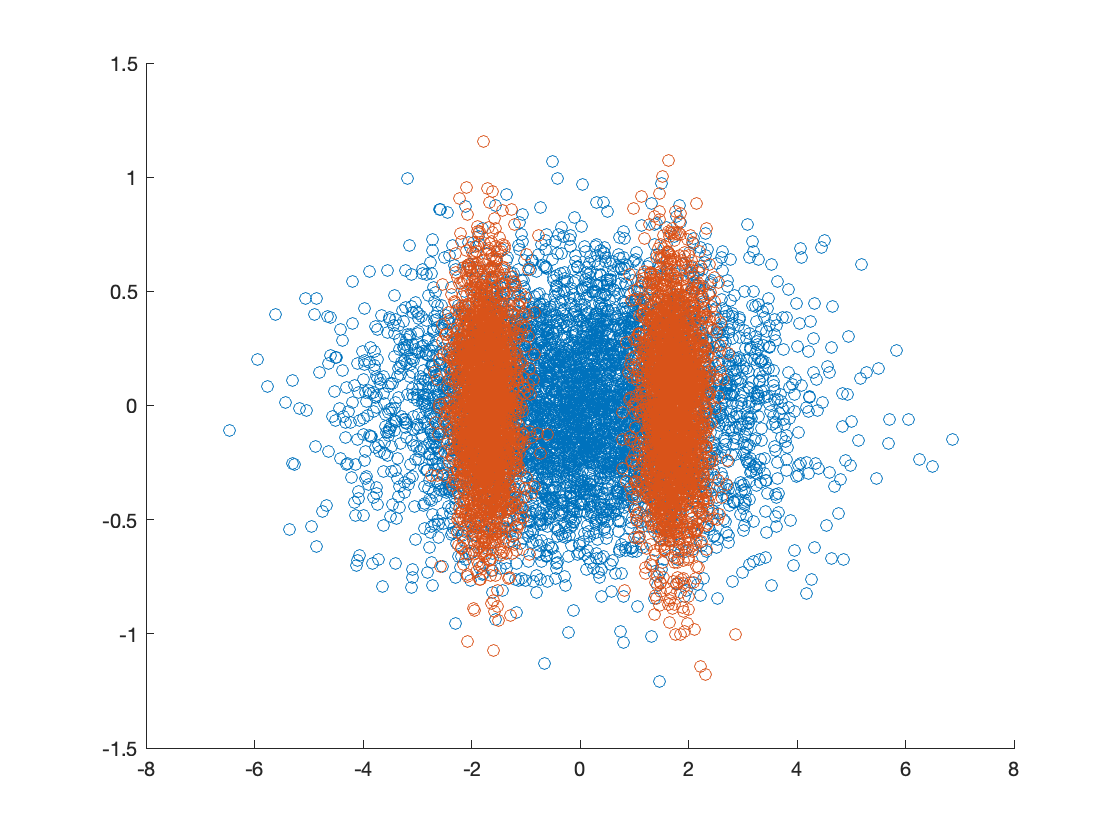
\includegraphics[width=\linewidth]{figures/exp1-1/pca.png}
				\caption{\label{fig:PCA} PCA}
			\end{subfigure}\hfill
			\begin{subfigure}[t]{0.24\linewidth}
				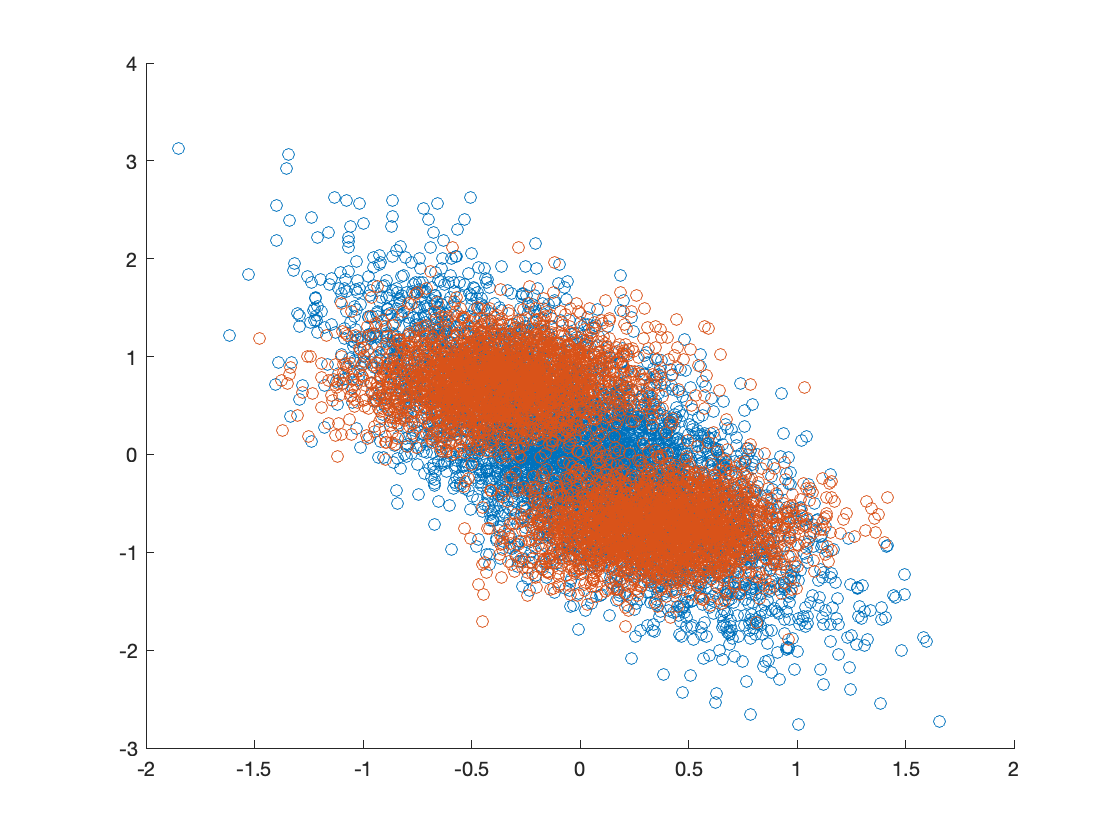
\includegraphics[width=\linewidth]{figures/exp1-1/fpca.png}
				\caption{\label{fig:FPCA} \textsc{FPCA} \cite{OA19}}
			\end{subfigure}\hfill
			\begin{subfigure}[t]{0.24\linewidth}
				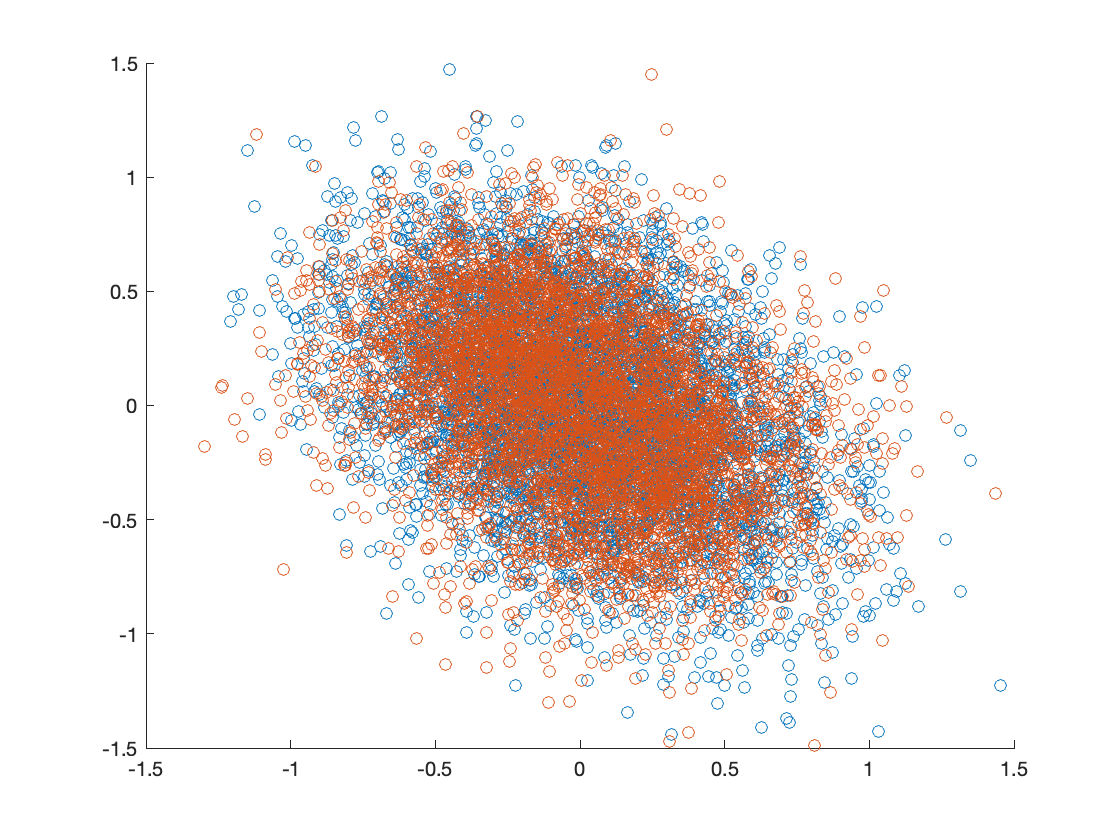
\includegraphics[width=\linewidth]{figures/exp1-1/mbfpca.png}
				\caption{\label{fig:ours} \textsc{MbF-PCA} (ours)}
			\end{subfigure}
			\caption{\label{fig:exp1-1} Synthetic data \#1: Comparison of PCA, FPCA, and \textsc{MbF-PCA} on data composed of two groups with same mean and covariance, but different distributions. Blue and orange represent different protected groups.}
		\end{center}
	\end{figure}
\end{frame}

\begin{frame}
	\frametitle{Synthetic data \#2}
	\begin{itemize}
		\item We consider a series of synthetic datasets of dimension $p$.
		
		\item For each $p$, the dataset is composed of two groups, each of size $n=240$ and sampled from two different $p$-variate normal distributions.
		
		\item We vary $p \in \{20, 30, \dots, 100\}$; see Section H of the SP \cite{Lee21} for a full description of the setting.
	\end{itemize}
\end{frame}

\begin{frame}
	\frametitle{Synthetic data \#2}
	\begin{figure}[!t]
		\begin{center}
			\begin{subfigure}[t]{0.49\columnwidth}
				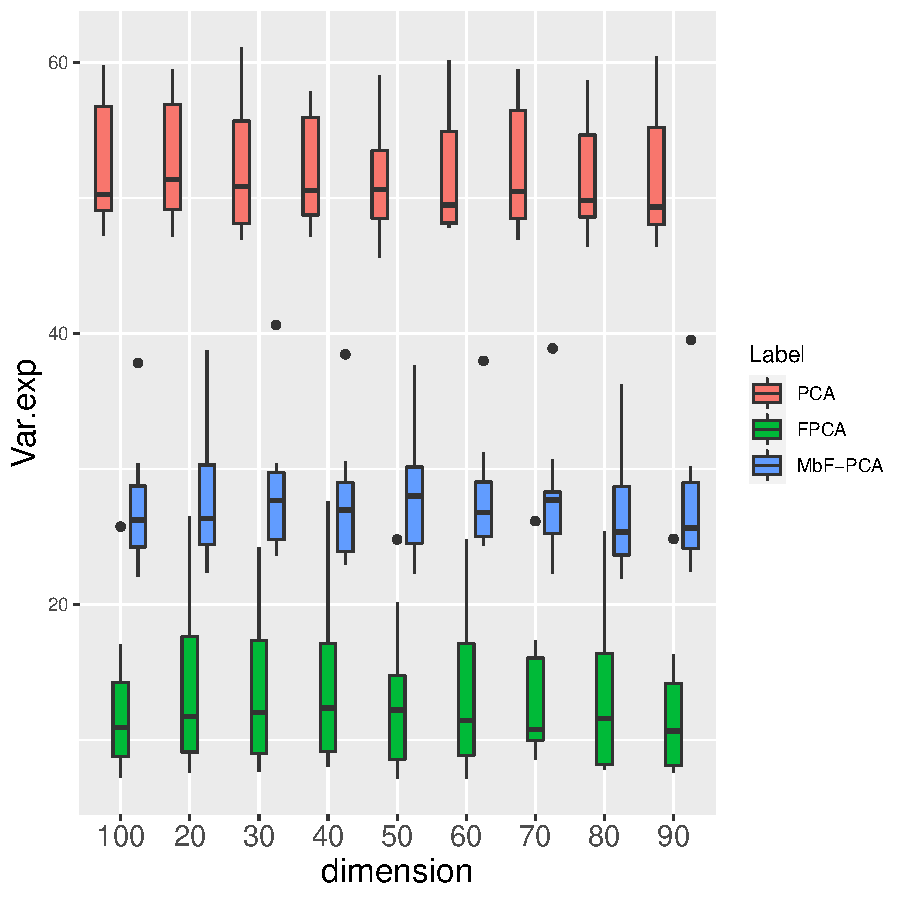
\includegraphics[width=\linewidth]{figures/exp1-2/varexp.pdf}
				\caption{\label{fig:varexp} Variance explained (\%)}
			\end{subfigure}
			\begin{subfigure}[t]{0.49\columnwidth}	
				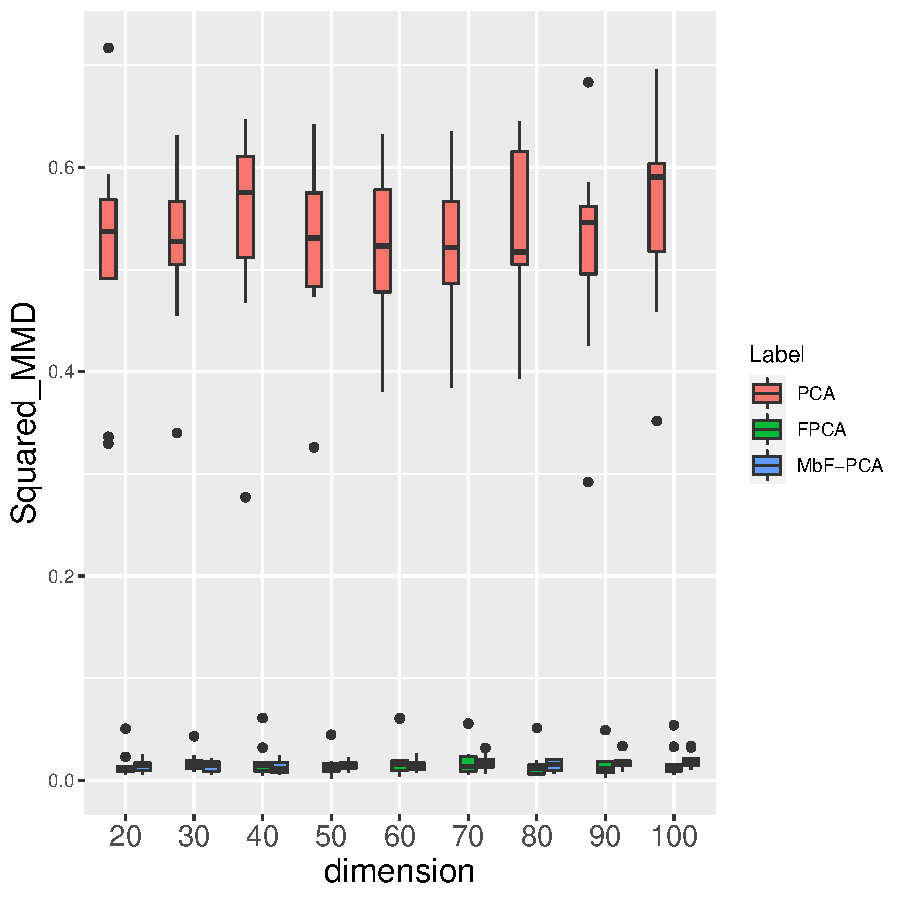
\includegraphics[width=\linewidth]{figures/exp1-2/mmd.pdf}
				\caption{\label{fig:mmd} $MMD^2$}
			\end{subfigure}
		\end{center}
		\caption{\label{fig:exp1-2} Synthetic data \#2: Comparison of PCA, FPCA, and \textsc{MbF-PCA} on the synthetic datasets of increasing dimensions.}
	\end{figure}
\end{frame}

\begin{frame}
	\frametitle{Synthetic data \#2}
	\begin{figure}
		\centering
		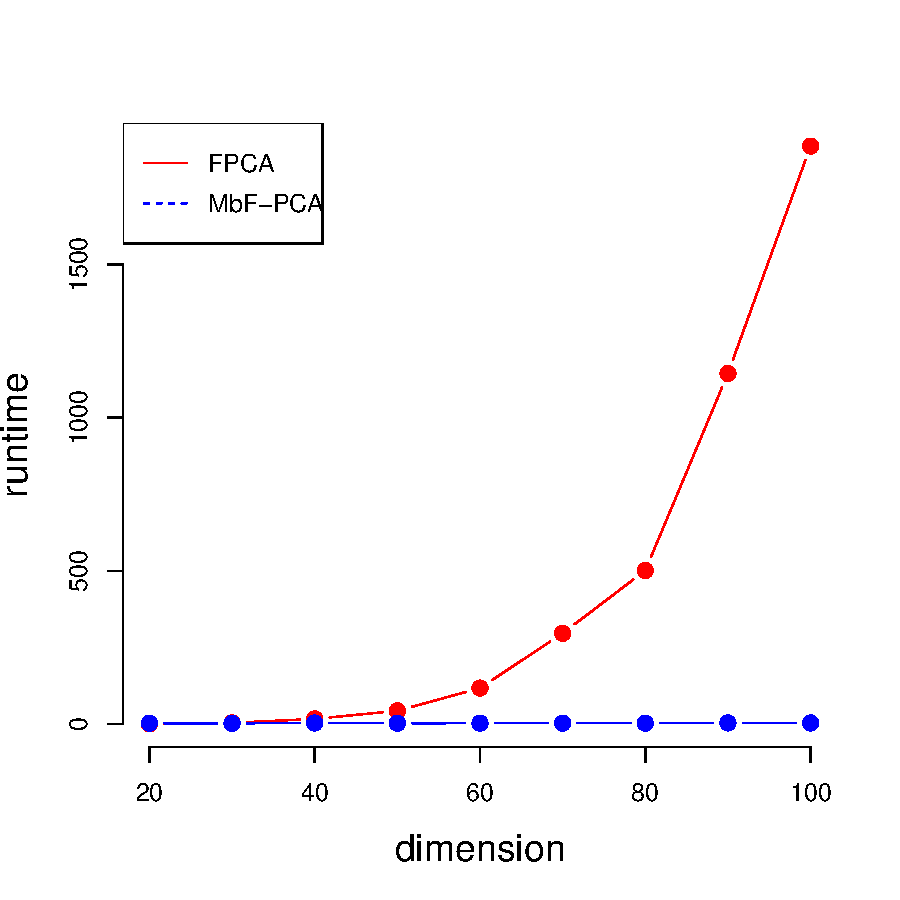
\includegraphics[width=0.5\linewidth]{figures/exp1-2/runtime.pdf}
		\caption{FPCA represents the SDP algorithm for fair PCA, and MbF-PCA represents our to-be introduced manifold-based algorithm for fair PCA. \cite{Lee21}}
		\label{fig:runtime}
	\end{figure}
\end{frame}

\begin{frame}
	\frametitle{UCI Datasets}
	\begin{itemize}
		\item We consider $3$ datasets from the UCI Repository \cite{UCI} (for pre-processing, we used AI Fairness 360 built-in functionalities \cite{aif360}):
		\begin{itemize}
			\item COMPAS dataset \cite{angwin2016machine}
			\begin{itemize}
				\item $n = 2468$, $p = 11$
				\item sensitive feature: ``race''
				\item downstream classification: ``crime again? (recidivism)''
			\end{itemize}
			
			\item German credit dataset
			\begin{itemize}
				\item $n = 1000$, $p = 57$
				\item sensitive feature: ``age''
				\item downstream classification: ``good credit class?''
			\end{itemize}
			
			\item Adult income dataset
			\begin{itemize}
				\item $n = 2261$, $p = 99$
				\item sensitive feature: ``gender''
				\item downstream classification: ``income larger than 50K?''
			\end{itemize}
			
		\end{itemize}
	\end{itemize}
\end{frame}

\begin{frame}
	\frametitle{UCI Datasets}
	\begin{itemize}
		\item We compare our manifold-based MbF-PCA with the SDP-based approach and PCA, both in explained variance and fairness.
		\begin{itemize}
			\item We emphasize that the {\bf only} comparable approach for this problem is PCA and FPCA!
		\end{itemize}
	
		\item For fairness, we consider our proposed MMD-metric {\it and} downstream task fairness.
	\end{itemize}
\end{frame}


\begin{frame}
	\frametitle{UCI Datasets}
	\begin{figure}
		\centering
		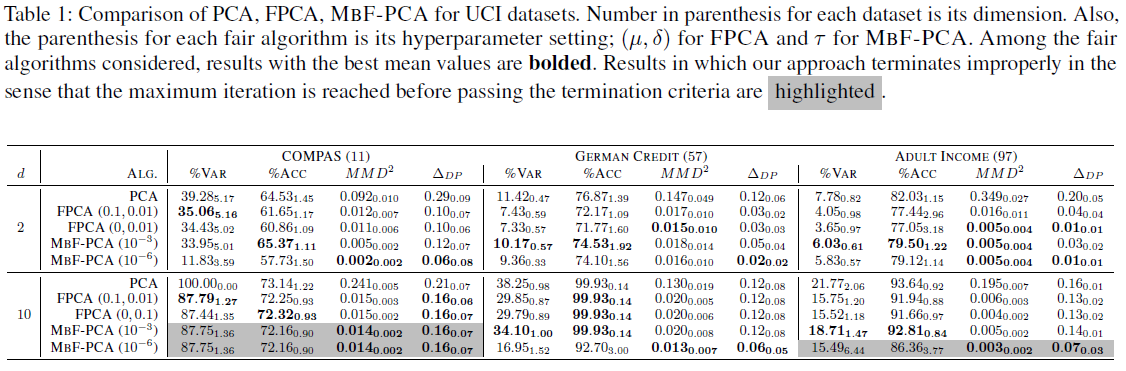
\includegraphics[width=\linewidth]{table.png}
	\end{figure}

	\begin{itemize}
		\item Across all considered datasets, \textsc{MbF-PCA} is shown to outperform \textsc{FPCA} in terms of fairness ($MMD^2$ and $\Delta_{DP}$) with low enough $\tau$.
		
		\item For \textsc{German Credit} and \textsc{Adult Income}, \textsc{MbF-PCA} shows a clear trade-off between explained variance and fairness; by relaxing $\tau$, we see that \textsc{MbF-PCA} outperforms \textsc{FPCA} in terms of explained variance and downstream task accuracy.
	\end{itemize}
\end{frame}


\begin{frame}
	\frametitle{UCI Datasets}
	\begin{itemize}
		\item Orthogonality of the PCs allows for us to {\it interpret} the PCs.
		\begin{itemize}
			\item This is part of a big set of techniques for interpretable ML, called {\bf exploratory data analysis (EDA)}
		\end{itemize}
		
		\item Communality of a feature is its variance contributed by the PCs \cite{multivariate-analysis}.
		\begin{itemize}
			\item This is computed as the sum of squares of the loadings of the considered feature.
		\end{itemize}
	
		\item It can be seen that the PCs resulting from
		MBF-PCA have the least correlations with age, the protected
		attribute.
	\end{itemize}
\end{frame}

\begin{frame}
	\frametitle{UCI Datasets}
	\begin{figure}[!t]
		\begin{center}
			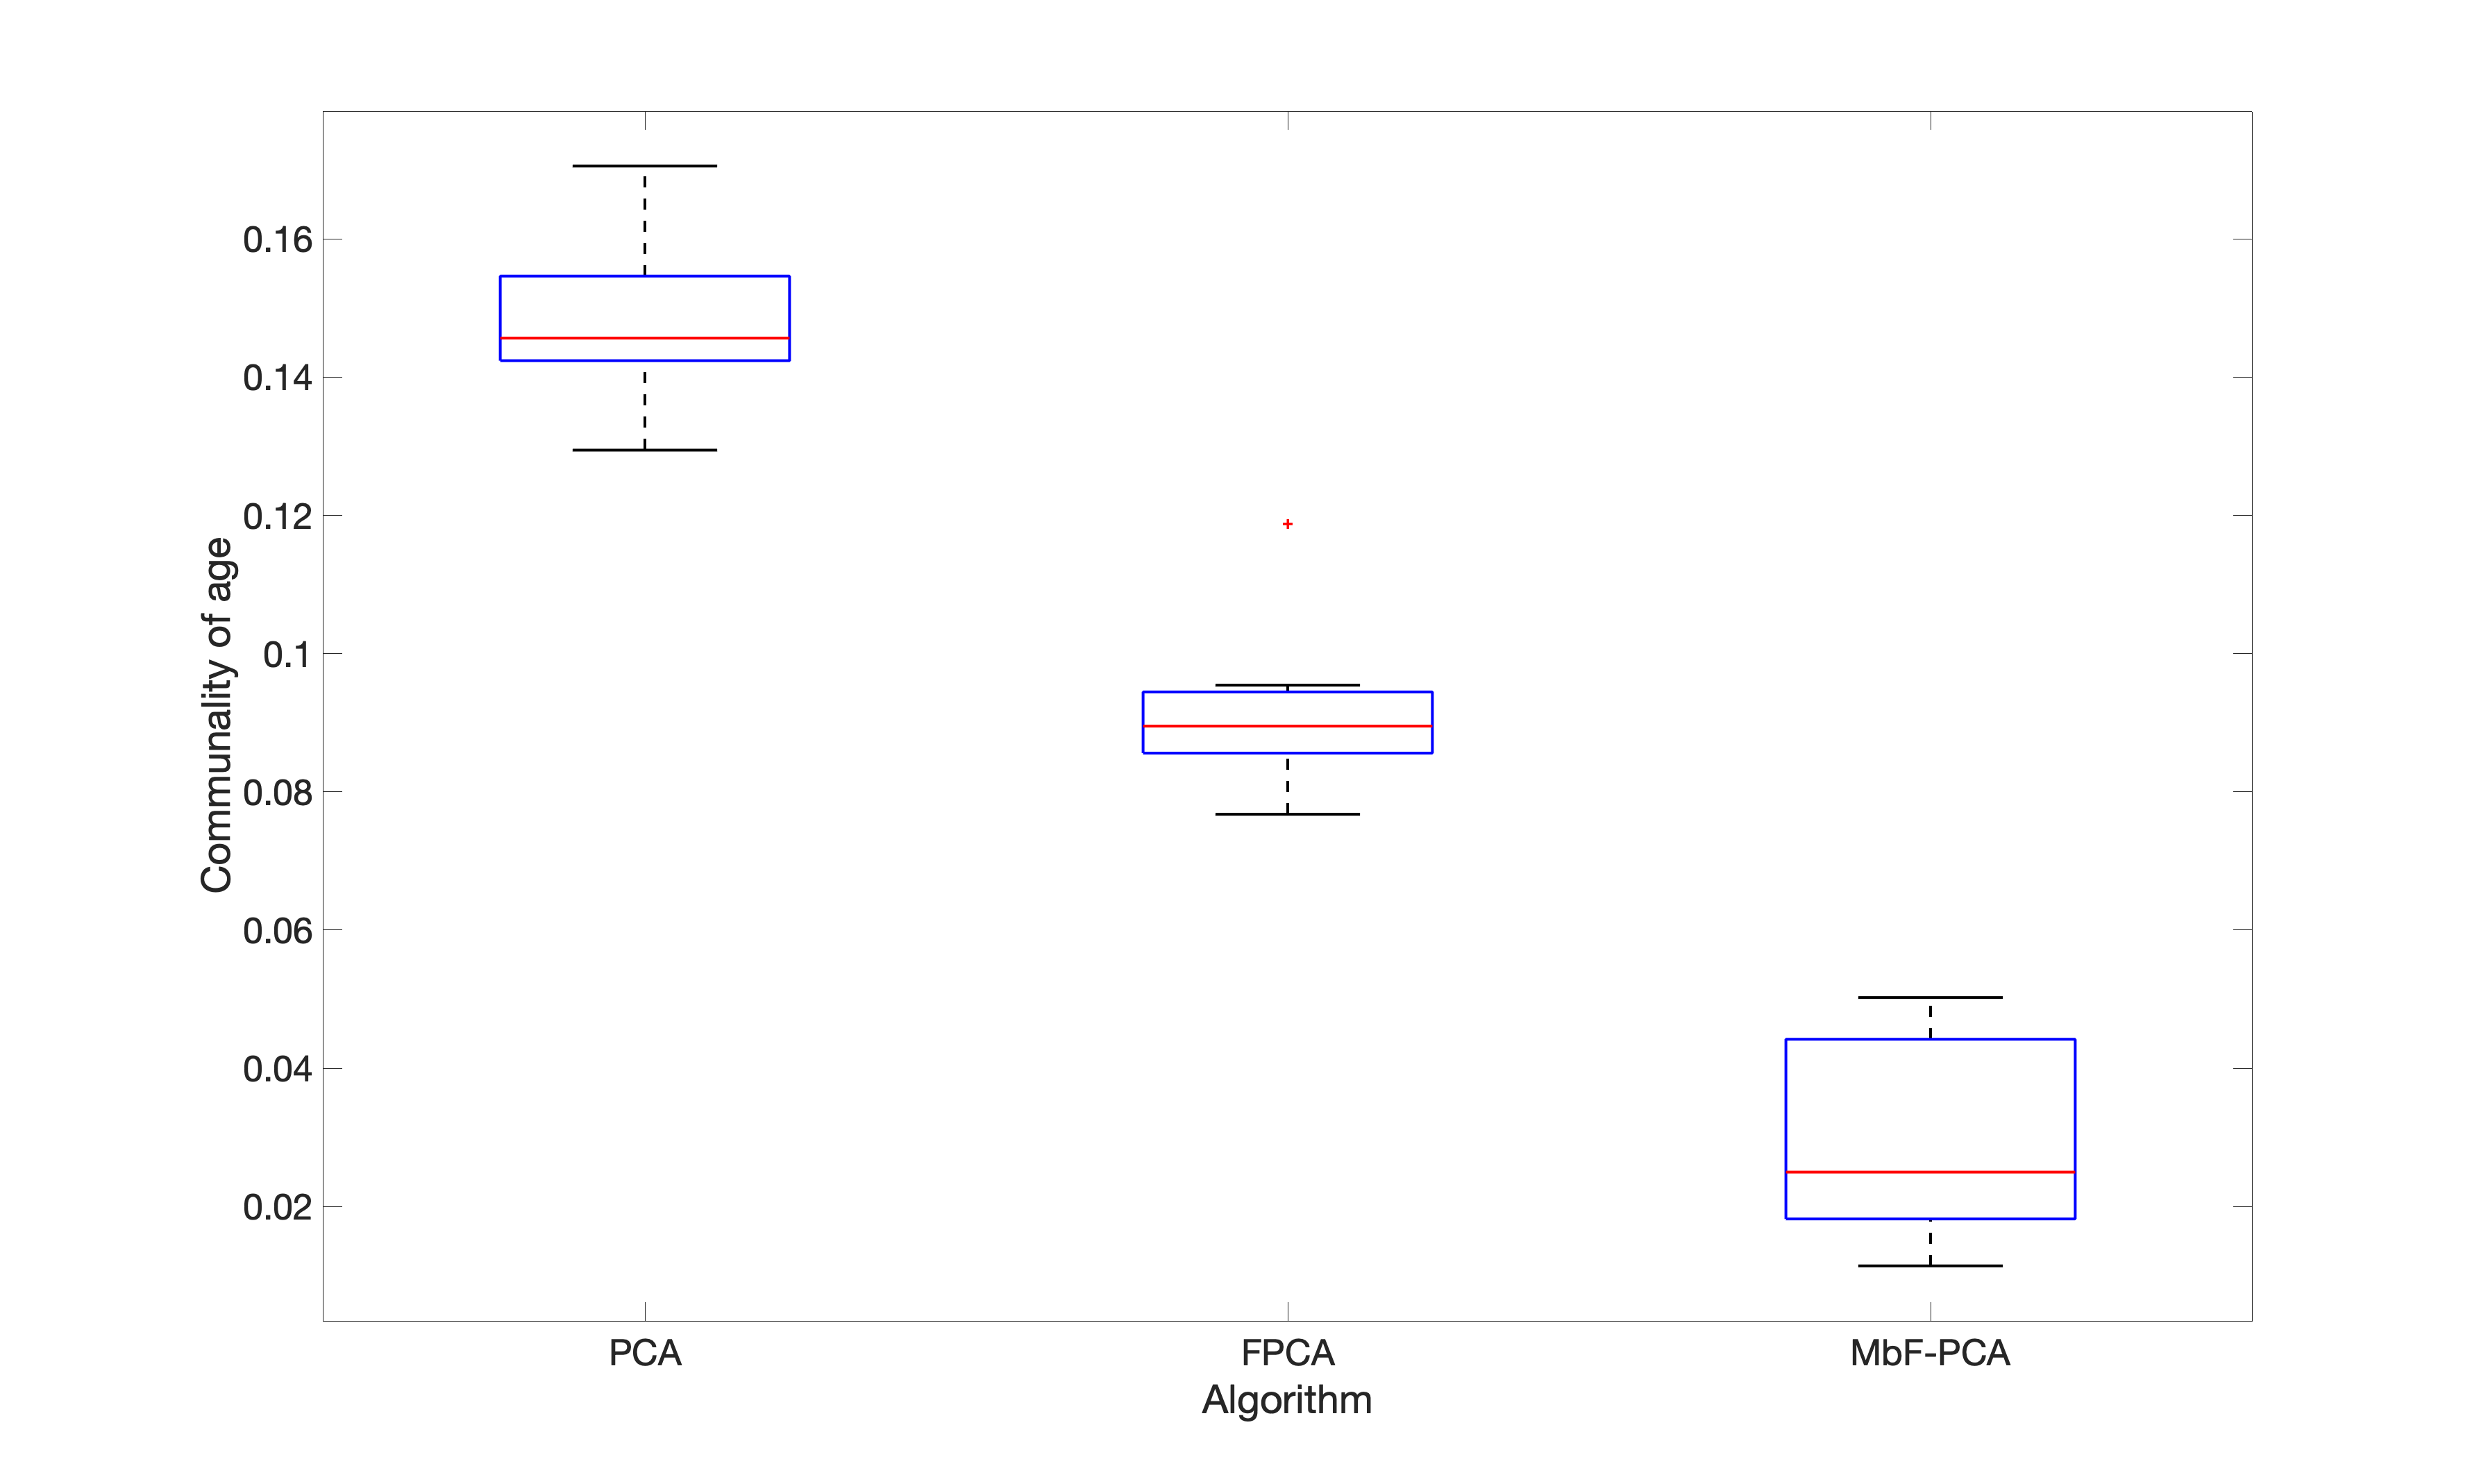
\includegraphics[width=0.8\linewidth]{figures/exp2-2/eda_german.png}
		\end{center}
		\caption{\label{fig:exp2-2-eda} Comparison of communality of ``age" of German credit dataset for PCA, \textsc{FPCA}, and \textsc{MbF-PCA}.}
	\end{figure}
\end{frame}


\begin{frame}
	\frametitle{Low Explained Variance of FPCA (*)}
	\begin{itemize}
		\item We analyze why this occurs using \textsc{German credit dataset}.
		
		\item Empirically, we observe that the leakage of explained variance occurs due to the relaxed rank constraint.
		
		\item Theoretically, under Gaussian assumption, we show that this is due to the relaxed rank constraint and the complicated effect of covariance constraint. (See Section C of the SP \cite{Lee21} for details)
	\end{itemize}
\end{frame}

\begin{frame}
	\frametitle{Low Explained Variance of FPCA (*)}
	\begin{figure}[!t]
		\begin{center}
			\begin{subfigure}[t]{0.49\linewidth}
				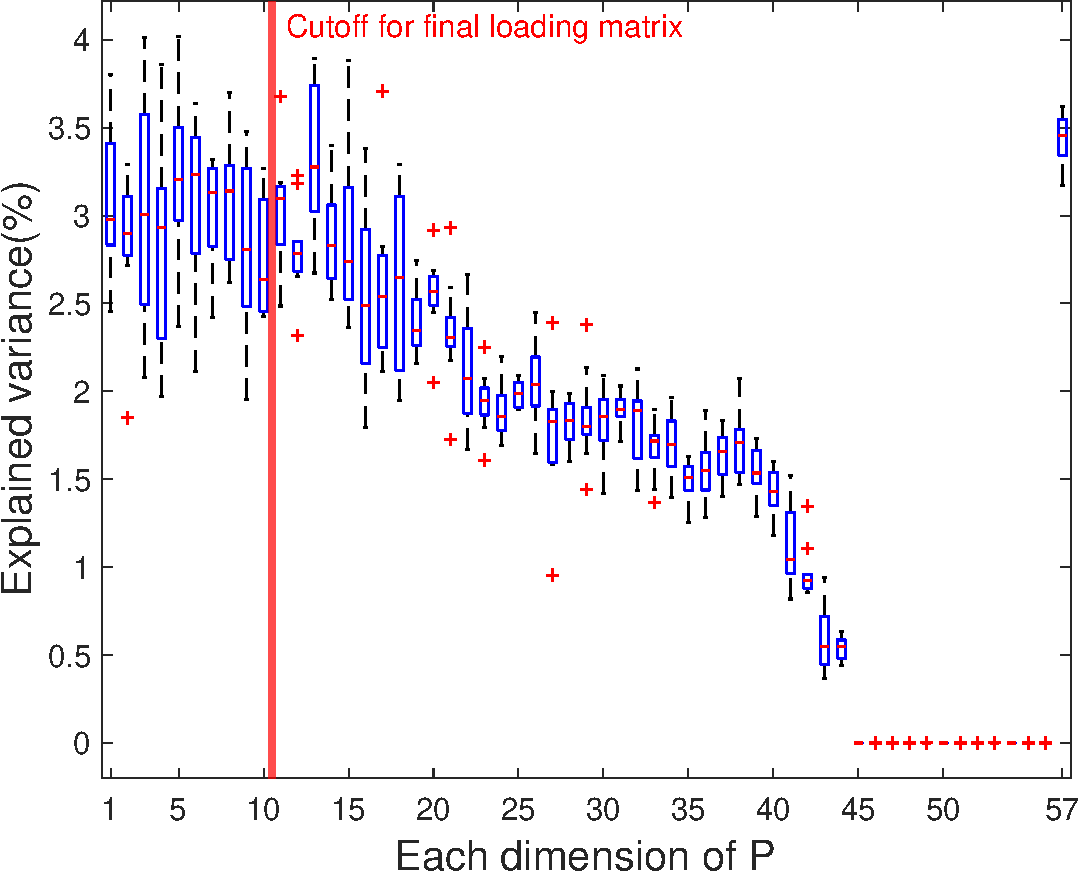
\includegraphics[width=\linewidth]{figures/supp/german_fpca.pdf}
				\caption{\label{fig:original} \textsc{FPCA} \cite{OA19}}
			\end{subfigure}\hfill
			\begin{subfigure}[t]{0.49\linewidth}
				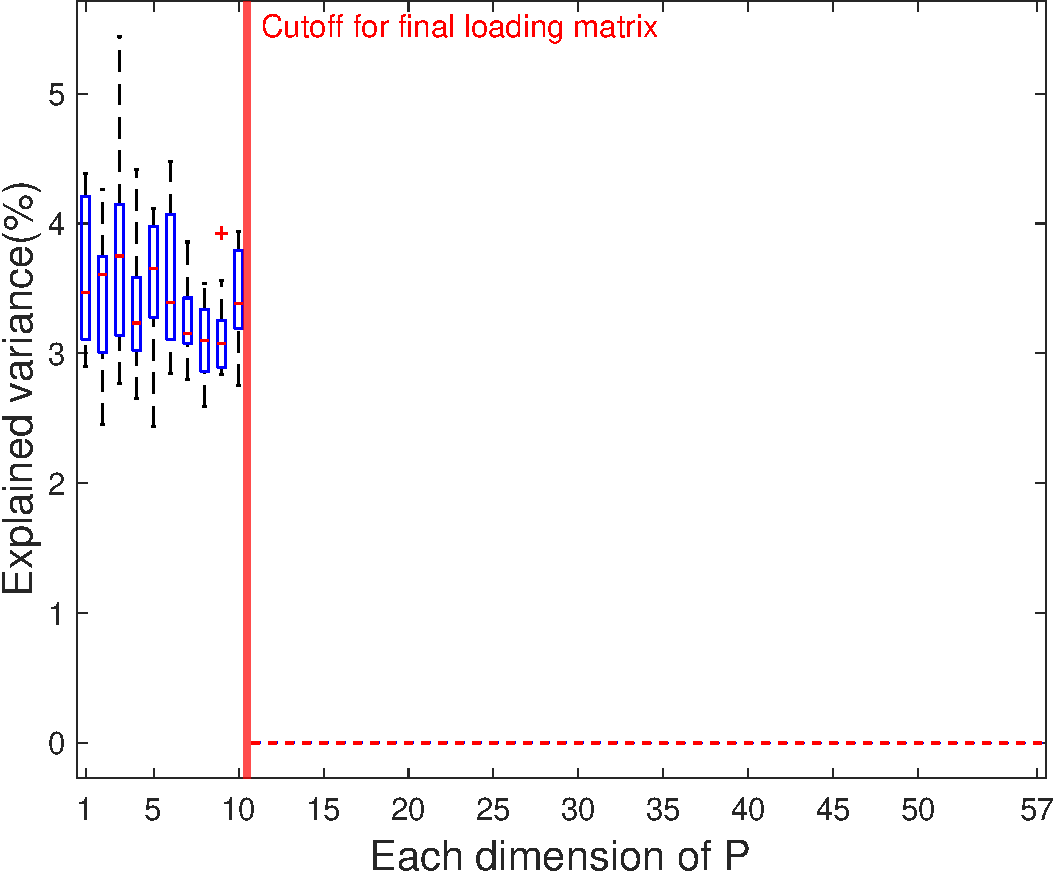
\includegraphics[width=\linewidth]{figures/supp/german_stfpca.pdf}
				\caption{\label{fig:PCA} \textsc{MbF-PCA} (ours)}
			\end{subfigure}
			\caption{\label{fig:low-sdp} Explained variance of each eigenvector of $P^*$ for \textsc{German credit dataset}, over the considered $10$ train-test splits.
				Note how in \textsc{FPCA}'s case, the there's significant ``leakage" of explained variance in the latter part (i.e. starting from $11$-th eigenvector of $P$)}
		\end{center}
	\end{figure}
\end{frame}


%---------------------------------------------------------

\section{Conclusion/Future works}

\begin{frame}
	\frametitle{Conclusion}
	\begin{itemize}
		\item {\bf New definition} for fair PCA based on MMD.
		
		\item Theoretical discussions on why our definition is more desirable than the previous one \cite{OA19}.
		
		\item MbF-PCA, a {\bf new manifold optimization framework} for fair PCA, along with theoretical discussions on why this approach is more favorable than the previous SDP-based approach \cite{OA19}.
		
		\item Provide new theoretical(optimality) guarantees of REPMS in both ideal and practical hyperparameter setting, extending previous results.
		
		\item Empirically, we show the efficacy of our algorithm on synthetic and UCI datasets in explained variance, fairness, and runtime.
	\end{itemize}
\end{frame}

\begin{frame}
	\frametitle{Future works}
	\begin{itemize}
		\item Statistical characterizations of our fair PCA in asymptotic regime, as well as incorporation of sparsity \cite{JL09}
		
		\item Incorporating stochastic optimization-type modifications \cite{Shamir15, fairbatch}
		\begin{itemize}
			\item This particularly important because our current approach scales quadratically in the number of data points as the computation of $MMD^2$ requires the full kernel gram matrix.
		\end{itemize}
	
		\item Further exploration into the interpretation of fair loading matrix.
	\end{itemize}
\end{frame}

\begin{frame}{}
	\centering \Large
	\emph{Thank you for your attention! Any questions?}
\end{frame}

\section{References}

%---------------------------------------------------------

%---------------------------------------------------------

\begin{frame}[allowframebreaks]
	\frametitle{References}
	\bibliographystyle{amsalpha}
	\bibliography{references.bib}
\end{frame}

%---------------------------------------------------------
	
\end{document}